%%%%%%%%%%%%%%%%%%%%%%%%%%%%%%%%%%%%%%%%%%%%%%%%%%%%%%%%%%%%%%%%%%%%%%%%%%%%%%%%
%%  LaTeX manuscript for SPIIRAS Proceedings
%%  Acamind: An Intelligent Academic Question Answering System
%%  charset=utf-8
%%%%%%%%%%%%%%%%%%%%%%%%%%%%%%%%%%%%%%%%%%%%%%%%%%%%%%%%%%%%%%%%%%%%%%%%%%%%%%%%

\documentclass[10pt]{SPIIRAS_Proceedings}

\usepackage{booktabs}
\usepackage{tabularx}
\usepackage{array}
\graphicspath{{figures/}{../figures/}}

% Float layout optimization to prevent giant white gaps on A5 paper
\renewcommand{\topfraction}{0.95}
\renewcommand{\bottomfraction}{0.85}
\renewcommand{\textfraction}{0.08}
\renewcommand{\floatpagefraction}{0.75}
\setcounter{topnumber}{3}
\setcounter{bottomnumber}{2}
\setcounter{totalnumber}{4}

% Correct Algorithm numbering and heading (remove erroneous comma)
\makeatletter
\renewenvironment{algorithm}[1][\unskip]{%
  \refstepcounter{alg}%
  \vskip 6pt\noindent%
  {\slshape Algorithm~\thealg\ifx\relax#1\relax\else\ (#1)\fi.}%
  \par\nopagebreak\smallskip\upshape
}{\par\vskip 6pt}
\makeatother

\usepackage{indentfirst}

% Format Section as standalone block heading on its own line (not run-in)
\titleformat{\section}[block]{\normalfont\normalsize\bfseries}{\thesection.}{.5em}
{\normalfont\normalsize\bfseries#1}
\titlespacing*{\section}
{\parindent}{8pt plus 2pt minus 2pt}{4pt plus 1pt minus 1pt}

\begin{document} 

\udk{006.72}
\titleEng{Acamind: An Intelligent Academic Question Answering System Integrating Retrieval-Augmented Generation and Hybrid Search for the Psychology Domain}
\authorsTitleEng{D.T.H. Chi, L.D. Tuan, N.C. Binh, N.V. Hung}
\authorsEng{Dinh Thi Hue Chi, Le Dinh Tuan, Nguyen Cong Binh, Nguyen Viet Hung.}

\abstractEng{
The rapid expansion of scientific literature in psychology poses severe challenges for manual literature lookup, while general Large Language Models (LLMs) suffer from factual hallucinations and a lack of verifiable source attribution. In clinical and academic disciplines, ungrounded assertions present unacceptable risks. This study introduces Acamind, a specialized Retrieval-Augmented Generation (RAG) assistant tailored to complex Vietnamese and international psychology literature. The system integrates a multi-engine PDF parsing pipeline with automated scan detection, parallel hybrid retrieval combining dense semantic representations (multilingual-e5-base on HNSW graphs) and sparse lexical search (Okapi BM25 on PostgreSQL GIN indexes) fused via Reciprocal Rank Fusion (RRF), a dynamic Confident Skip reranking algorithm, and strict non-parametric prompt enforcement for Llama 3.3 70B. Empirical evaluation across a live pilot of real academic queries demonstrated a Faithfulness score of 1.00, an Answer Relevancy of 1.00, and a Context Quality score of 0.867 under automated LLM-as-a-judge evaluation (Gemini 3.1 Flash-Lite). Stress testing across 1,000 operational scenarios confirmed a 98.8\% overall benchmark pass rate, maintaining an average system latency of 2.39 seconds. An active circuit-breaker mechanism safely rejects unparseable scanned documents in 1.50 seconds with zero hallucinated output. These results establish an empirical foundation for dependable, verifiable AI research assistants in specialized academic disciplines.
}

\keywordsEng{Retrieval-Augmented Generation, RAG, Hybrid Search, Academic Question Answering, Psychology Domain, Natural Language Processing, Hallucination Control.}

\makeengtitle

\normalsize

\section{Introduction}\label{sec:introduction}
Modern academic research in psychology, behavioral science, and clinical psychiatry is characterized by an exponential influx of scientific monographs, therapy manuals, and empirical trial reports. In higher education environments such as Vietnam, university students, postgraduate researchers, and clinical practitioners rely predominantly on massive, complex digital repositories distributed as raw PDF textbooks and regulatory clinical protocols \cite{iancarelli2025affective}. Navigating these multi-hundred-page documents using conventional keyword-matching or lexical search tools is increasingly inefficient, as standard search fails to bridge semantic synonymy, resolve theoretical concepts, or perform cross-document synthesis.

The rapid adoption of Large Language Models (LLMs) has expanded possibilities for automated scientific question answering and literature analysis. However, deploying general-purpose LLMs directly into specialized clinical and academic disciplines is severely impeded by the phenomenon of ``hallucination''---the generation of plausible yet factually incorrect or ungrounded assertions \cite{min2023factscore, lu2026mhb}. In clinical psychology, diagnostic classification, and psychopharmacological guidance, unverified statements lacking precise source attribution introduce grave risks of misinterpretation and harm.

To circumvent parametric hallucination, contemporary research has embraced Retrieval-Augmented Generation (RAG) \cite{lewis2020retrieval}. Nevertheless, current off-the-shelf RAG baselines encounter three critical bottlenecks when confronted with real-world academic literature:
\begin{enumerate}
    \item \textit{Complex PDF Ingestion Bottleneck:} Academic textbooks feature multi-column typesetting, complex data tables, non-standard embedded fonts, and interspersed scanned pages. Naive text splitting damages reading continuity, fragments tabular relationships, and causes unparseable image text to leak into the prompt \cite{elbachyr2024empirical, santos2026pdf}.
    \item \textit{Vocabulary Mismatch in Specialized Retrieval:} Pure dense vector models (e.g., DPR, standard sentence transformers) capture general semantic intent but frequently miss exact diagnostic nomenclature, specialized abbreviations, or numerical criteria (such as DSM-5 diagnostic codes or pharmacological dosages). Conversely, sparse lexical methods (such as BM25) capture exact terms but fail on conceptual paraphrasing \cite{karpukhin2020dense, formal2021splade}.
    \item \textit{Absence of Page-Level Traceable Citations:} Existing academic QA systems either generate generic summaries or reference broad document IDs without specifying exact page locations, preventing rapid manual verification by human clinicians and researchers.
\end{enumerate}
To date, there is a distinct absence of an end-to-end, domain-optimized RAG system capable of autonomously handling multi-page Vietnamese and international psychology textbooks, executing hybrid retrieval, and delivering answers backed by verifiable page-level anchor citations.

To address these fundamental limitations, this paper presents \textbf{Acamind}, an intelligent academic question-answering architecture developed specifically for the psychology domain. Acamind establishes a closed-loop processing pipeline that integrates: (i) an adaptive multi-parser ingestion engine with automatic scan detection; (ii) a parallel hybrid retrieval mechanism combining dense HNSW vector search \cite{wang2022text, malkov2020efficient} and sparse GIN lexical search \cite{formal2021splade} via Reciprocal Rank Fusion (RRF) \cite{cormack2009reciprocal}; (iii) a dynamic Confident Skip reranking algorithm that bypasses heavy cross-encoders when the top candidate is highly dominant; and (iv) a strict non-parametric generation controller paired with an automated circuit-breaker for safe refusal.

The principal contributions of this work are summarized as follows:
\begin{itemize}
    \item \textbf{End-to-End Specialized Architecture:} We design and deploy a four-layer RAG architecture that resolves layout fragmentation across complex psychology textbooks and provides transparent page-level anchor citations ([File.pdf - Page X]).
    \item \textbf{Latency-Optimized Hybrid Retrieval:} We introduce a Confident Skip decision boundary ($\Delta \text{RRF} \ge 2.5$) that dynamically bypasses cross-attention reranking, eliminating $200\text{ms}-500\text{ms}$ of computational overhead while maintaining top-rank precision.
    \item \textbf{Rigorous Empirical Validation:} We validate Acamind across a live pilot of real academic queries ($N=10$) using the RAGAS framework (achieving Faithfulness = 1.00, Relevancy = 1.00, Context Quality = 0.867) and benchmark system robustness across 1,000 operational test scenarios with a 98.8\% pass rate.
\end{itemize}

The remainder of this paper is organized as follows. Section~\ref{sec:related_work} reviews foundational literature on academic QA benchmarks, dense-sparse hybrid search, and automated RAG evaluation. Section~\ref{sec:methodology} delineates the proposed four-layer Acamind architecture, mathematical retrieval formulations, the Confident Skip reranking algorithm, and algorithmic complexity bounds. Section~\ref{sec:experiments} details the experimental setup, live academic pilot results, latency profiling, operational stress testing across 1,000 scenarios, baseline comparisons, and systematic ablation experiments across retrieval paradigms. Section~\ref{sec:discussion} discusses empirical hypotheses, noise filtering dynamics, and system generalizability. Finally, Section~\ref{sec:conclusion} concludes the paper and delineates future research directions.

\section{Related Work}\label{sec:related_work}

\subsection{Academic \& Biomedical Question Answering Benchmarks}
Benchmark datasets such as PubMedQA \cite{jin2019pubmedqa} and MedQuAD \cite{abacha2019question} have established standardized evaluation frameworks for biomedical inquiry. More recently, the Medical Hallucination Benchmark (MHB) \cite{lu2026mhb} introduced rigorous diagnostics for clinical factual consistency. However, existing datasets predominantly operate on pre-extracted short abstracts or curated snippet pairs, bypassing the real-world operational challenges of automated ingestion and retrieval directly from hundreds of pages of raw PDF literature. QASPER \cite{dasigi2021dataset} addressed full-paper reading but assumed the target document was already known and supplied in the prompt. Acamind bridges these gaps by providing an autonomous, repository-wide retrieval and synthesis engine over comprehensive psychology textbooks.

\subsection{Information Retrieval \& Dense-Sparse Fusion}
Dense Passage Retrieval (DPR) \cite{karpukhin2020dense}, ANCE \cite{xiong2021approximate}, and late-interaction architectures like ColBERT \cite{khattab2020colbert} demonstrated marked improvements in semantic relevance over lexical baselines. However, in domain-specific technical literature, dense retrievers frequently exhibit blind spots regarding rare psychiatric codes, drug names, and diagnostic thresholds. Sparse neural representations like SPLADE \cite{formal2021splade} and classic BM25 mitigate this vocabulary mismatch. Acamind leverages parallel dense-sparse execution unified by Reciprocal Rank Fusion (RRF) \cite{cormack2009reciprocal} to capture both deep semantic concepts and exact terminological tokens.

\subsection{Document Ingestion, Reranking \& Automated Evaluation}
Recent empirical investigations by El Bachyr et al. \cite{elbachyr2024empirical} and dos Santos et al. \cite{santos2026pdf} established that document structure extraction and chunking strategies dictate downstream RAG quality. Rather than relying on static single-parser chunkers, modern pipelines require table-aware extraction and scan identification. For factual assessment, the RAGAS framework \cite{es2024ragas} provides automated multi-dimensional evaluation (Faithfulness, Answer Relevancy, Context Precision) using LLM-as-a-judge methodologies, overcoming the prohibitive cost and latency of manual factual precision audits \cite{min2023factscore}. Acamind adapts these evaluation principles to measure factual grounding on live academic literature.

\subsection{Research Gap Synthesis}
Prior studies have largely treated PDF parsing, retriever optimization, and reranker latency in isolation. There remains an acute deficit of integrated, open architectures tailored to specialized Vietnamese psychology education that simultaneously resolve multi-page PDF ingestion, optimize multi-stage retrieval latency, and eliminate factual hallucination via verifiable page citations.

\begin{figure}[!t]
    \centering
    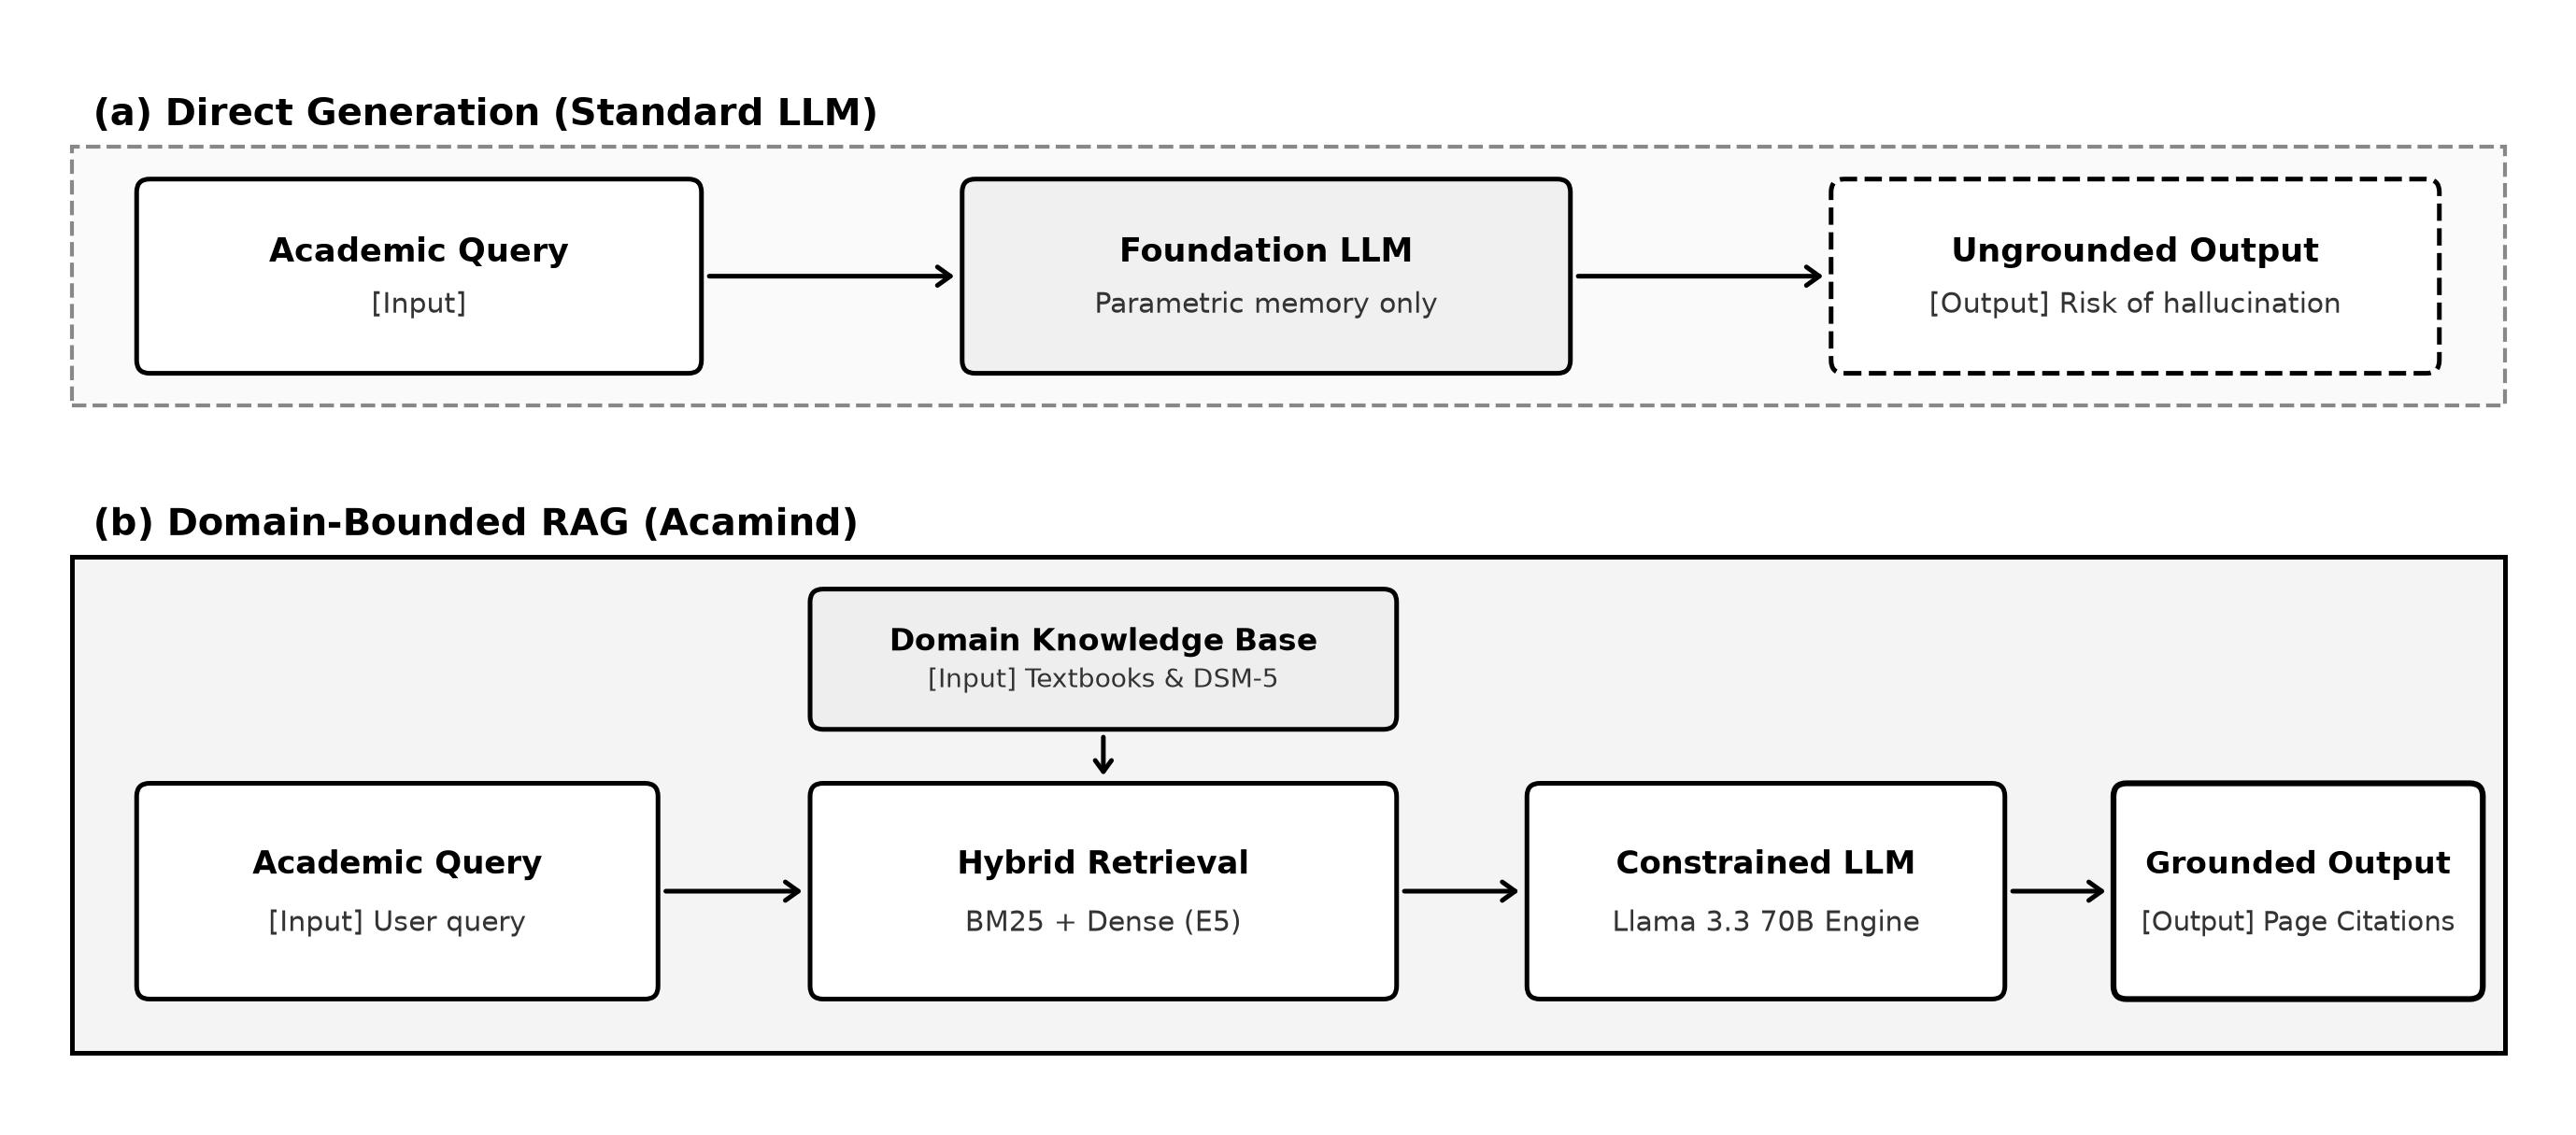
\includegraphics[width=0.95\textwidth]{figures/fig_rag_architecture.jpg}
    \caption{Conceptual Paradigm: Generic LLM Hallucination Risk vs. Acamind Domain-Specialized RAG System.}
    \label{fig:rag_diagram}
\end{figure}

\section{System Architecture and Methodology}\label{sec:methodology}
The core philosophy of Acamind is illustrated in Fig.~\ref{fig:rag_diagram}. Unlike generic LLMs that rely on ungrounded internal parameters, Acamind enforces context grounding, verifiable page attribution, and proactive refusal on unparseable inputs.

\subsection{System Overview}
The Acamind architecture is structured into four functional layers, depicted in Fig.~\ref{fig:architecture}:
\begin{enumerate}
    \item \textit{Knowledge Base Layer:} Stores digitized academic PDF textbooks, a Neo4j Graph Database for structural ontology and author-concept relationships, and L1 Compressed Memory containing high-level chapter summaries generated via Gemini.
    \item \textit{Preprocessing \& Chunking Layer:} Houses the PyMuPDF and pdfplumber multi-parser, a character-density scan detector, a recursive semantic character splitter (800-character chunk size, 200-character overlap), and SHA-256 deduplication.
    \item \textit{Storage Layer:} Built on PostgreSQL featuring pgvector with Hierarchical Navigable Small World (HNSW) indexing ($\mathit{ef}_{\text{search}}=100$) for 768-dimensional dense embeddings, paired with a Generalized Inverted Index (GIN) storing tsvector representations for Okapi BM25.
    \item \textit{Processing \& Generation Engine:} Coordinates parallel hybrid retrieval, RRF scoring, the Confident Skip reranker test, cross-attention scoring via BGE-Reranker-v2-m3, and generation via Llama 3.3 70B under a 10-rule system prompt.
\end{enumerate}

\begin{figure}[!t]
    \centering
    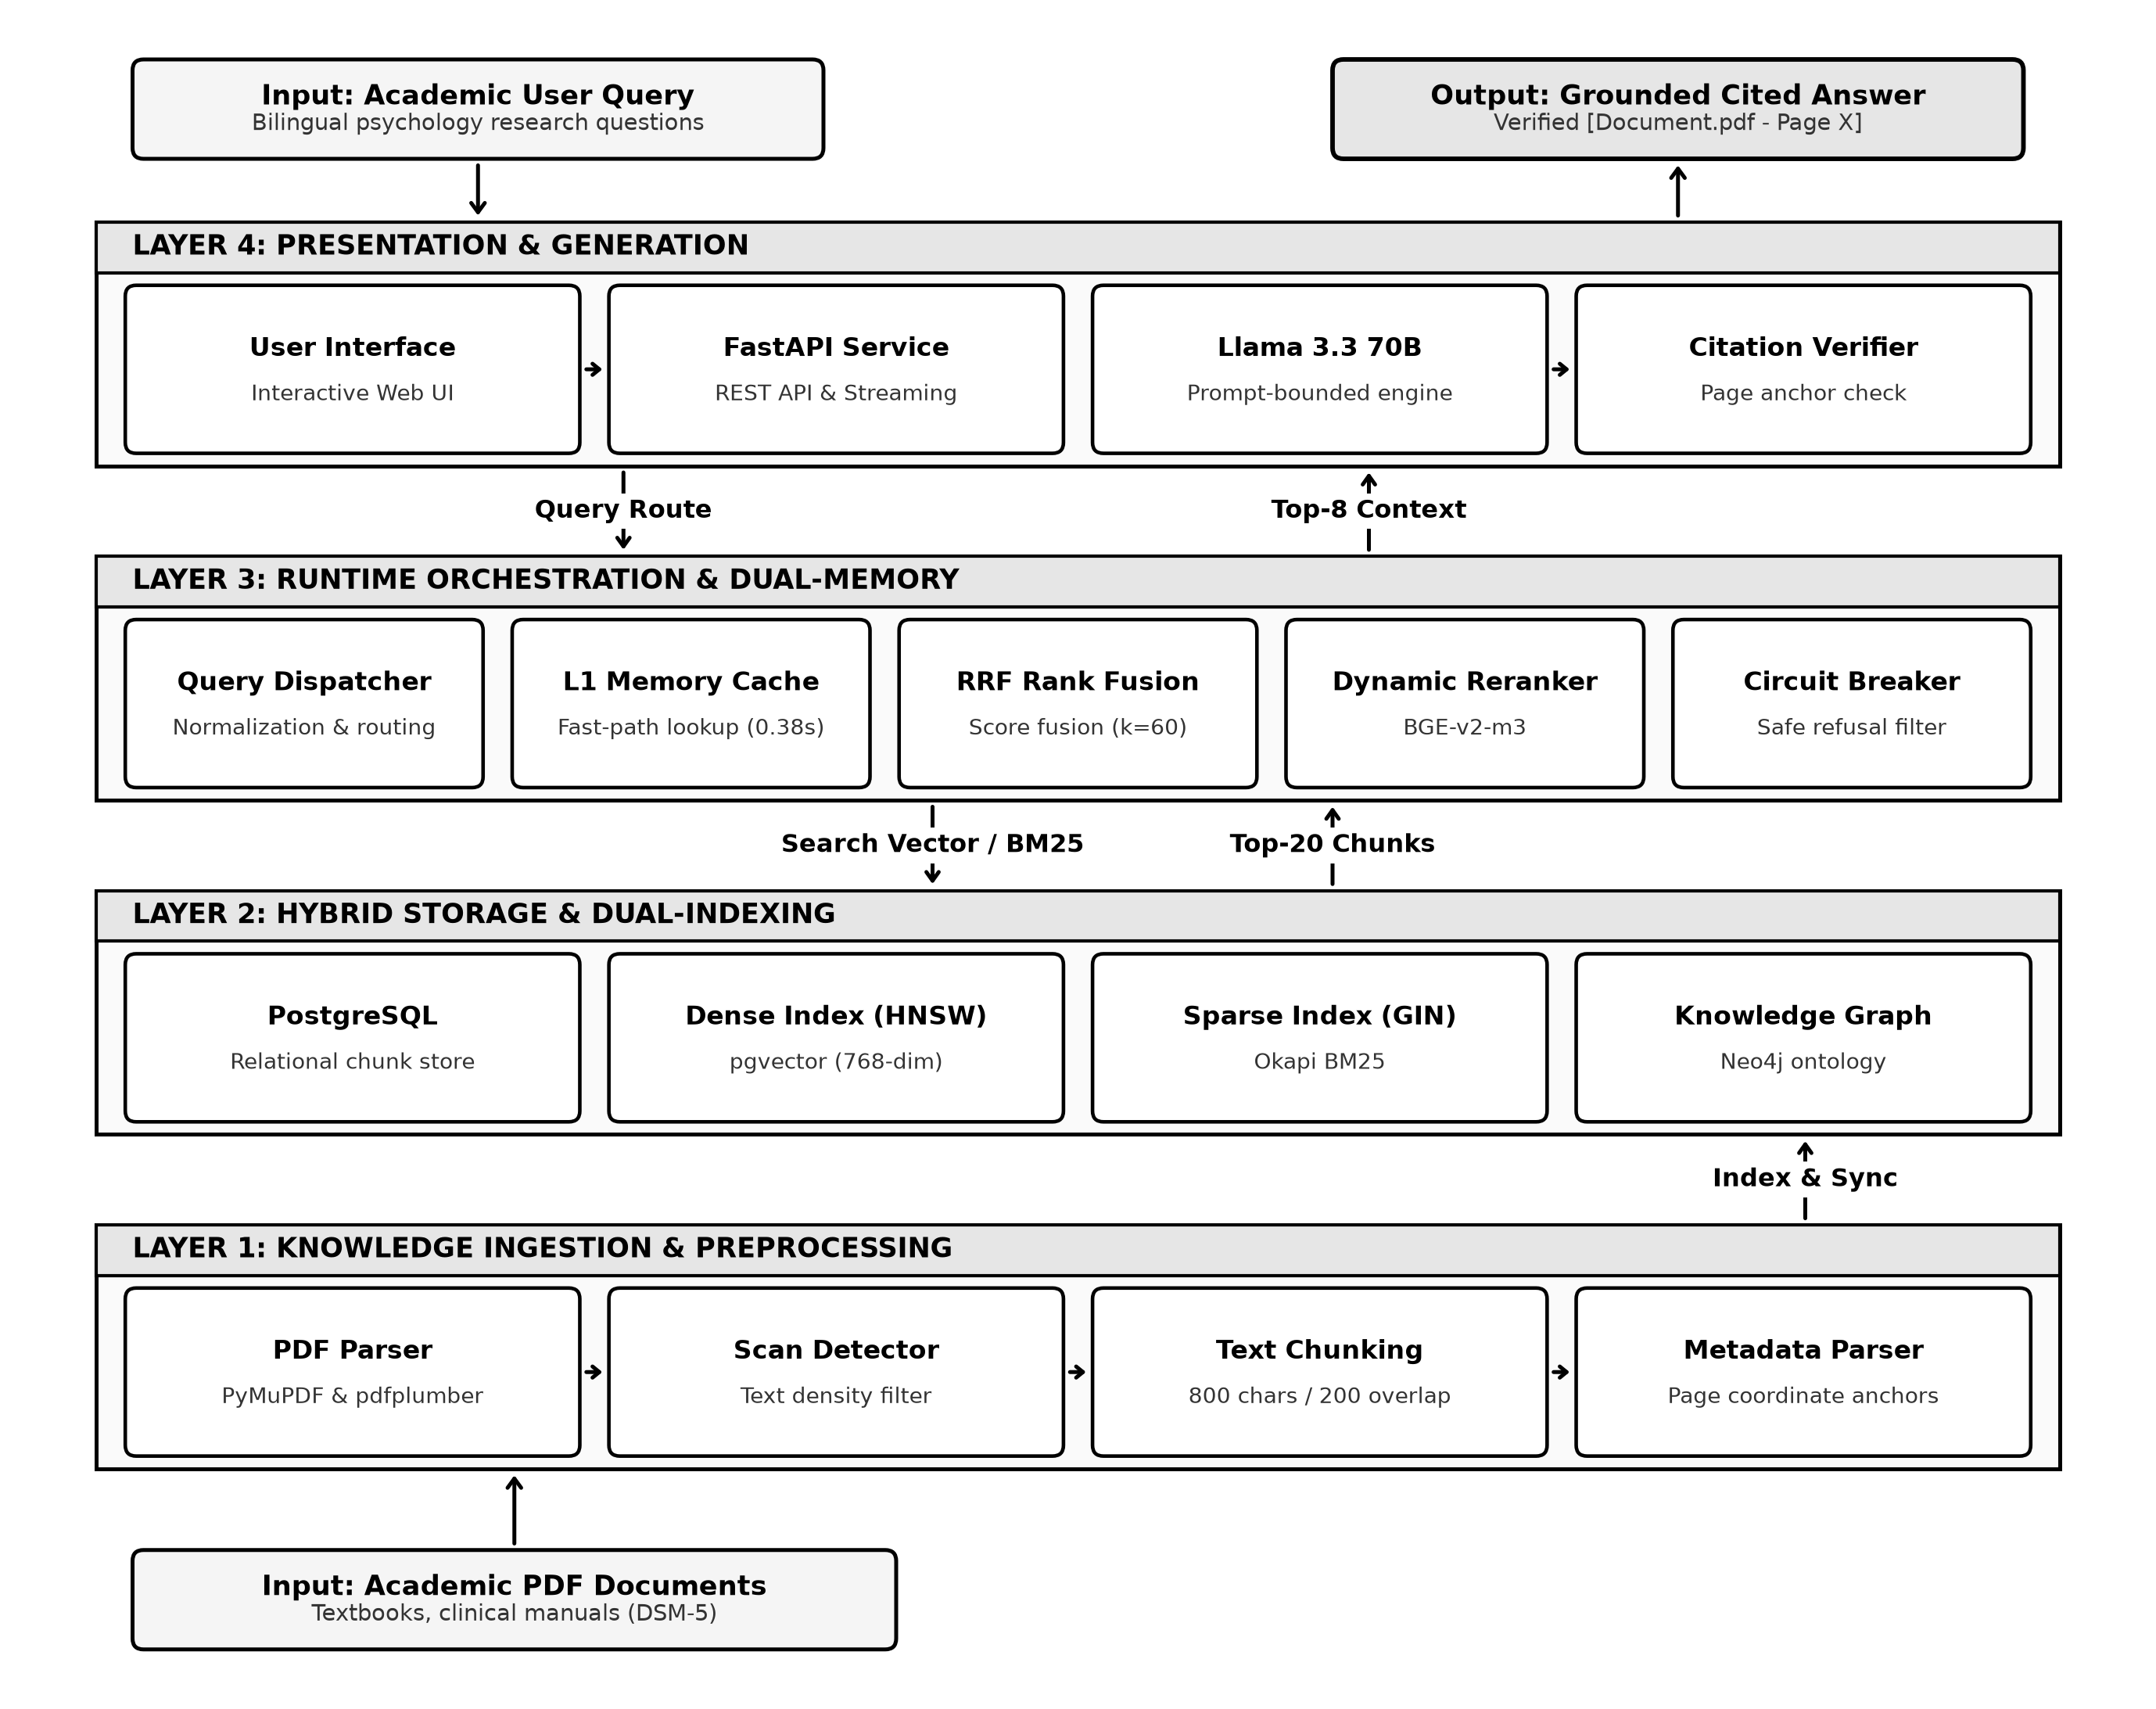
\includegraphics[width=0.88\textwidth]{figures/fig_architecture.png}
    \caption{End-to-End 4-Layer Architecture Blueprint of the Acamind System.}
    \label{fig:architecture}
\end{figure}

Mathematically, given an academic query $Q$, the conditional probability of synthesizing response sequence $Y = (y_1, \dots, y_N)$ over retrieved context candidate set $\mathcal{D} = \{d_1, \dots, d_k\}$ is formulated as:
\begin{equation}
P(Y | Q) = \sum_{d \in \mathcal{D}} P_R(d | Q) \prod_{i=1}^{N} P_G(y_i | Q, d, y_{<i})
\end{equation}
where $P_R(d | Q)$ is the joint retriever-reranker selection probability and $P_G$ denotes the autoregressive generation probability.

\subsection{Document Preprocessing \& Chunking}
Academic textbooks are parsed through a multi-tool extraction pipeline. PyMuPDF handles primary layout extraction, while pdfplumber serves as a specialized fallback for tabular and structured data. Pages exhibiting fewer than 50 text characters are automatically classified as scanned image pages, preventing blank extraction artifacts from degrading the index. Extracted text streams are segmented using a Recursive Character Text Splitter with chunk size $L=800$ characters and overlap $\Delta L=200$ characters, maintaining semantic continuity across paragraph boundaries. Document metadata (file title, chapter heading, and absolute page number $P$) is attached to every chunk.

\subsection{Parallel Hybrid Retrieval}
To maximize recall across conceptual and terminological queries, Acamind initiates simultaneous retrieval over dense and sparse representations, as shown in Fig.~\ref{fig:pipeline_hybrid_rerank}:

\begin{figure}[!t]
    \centering
    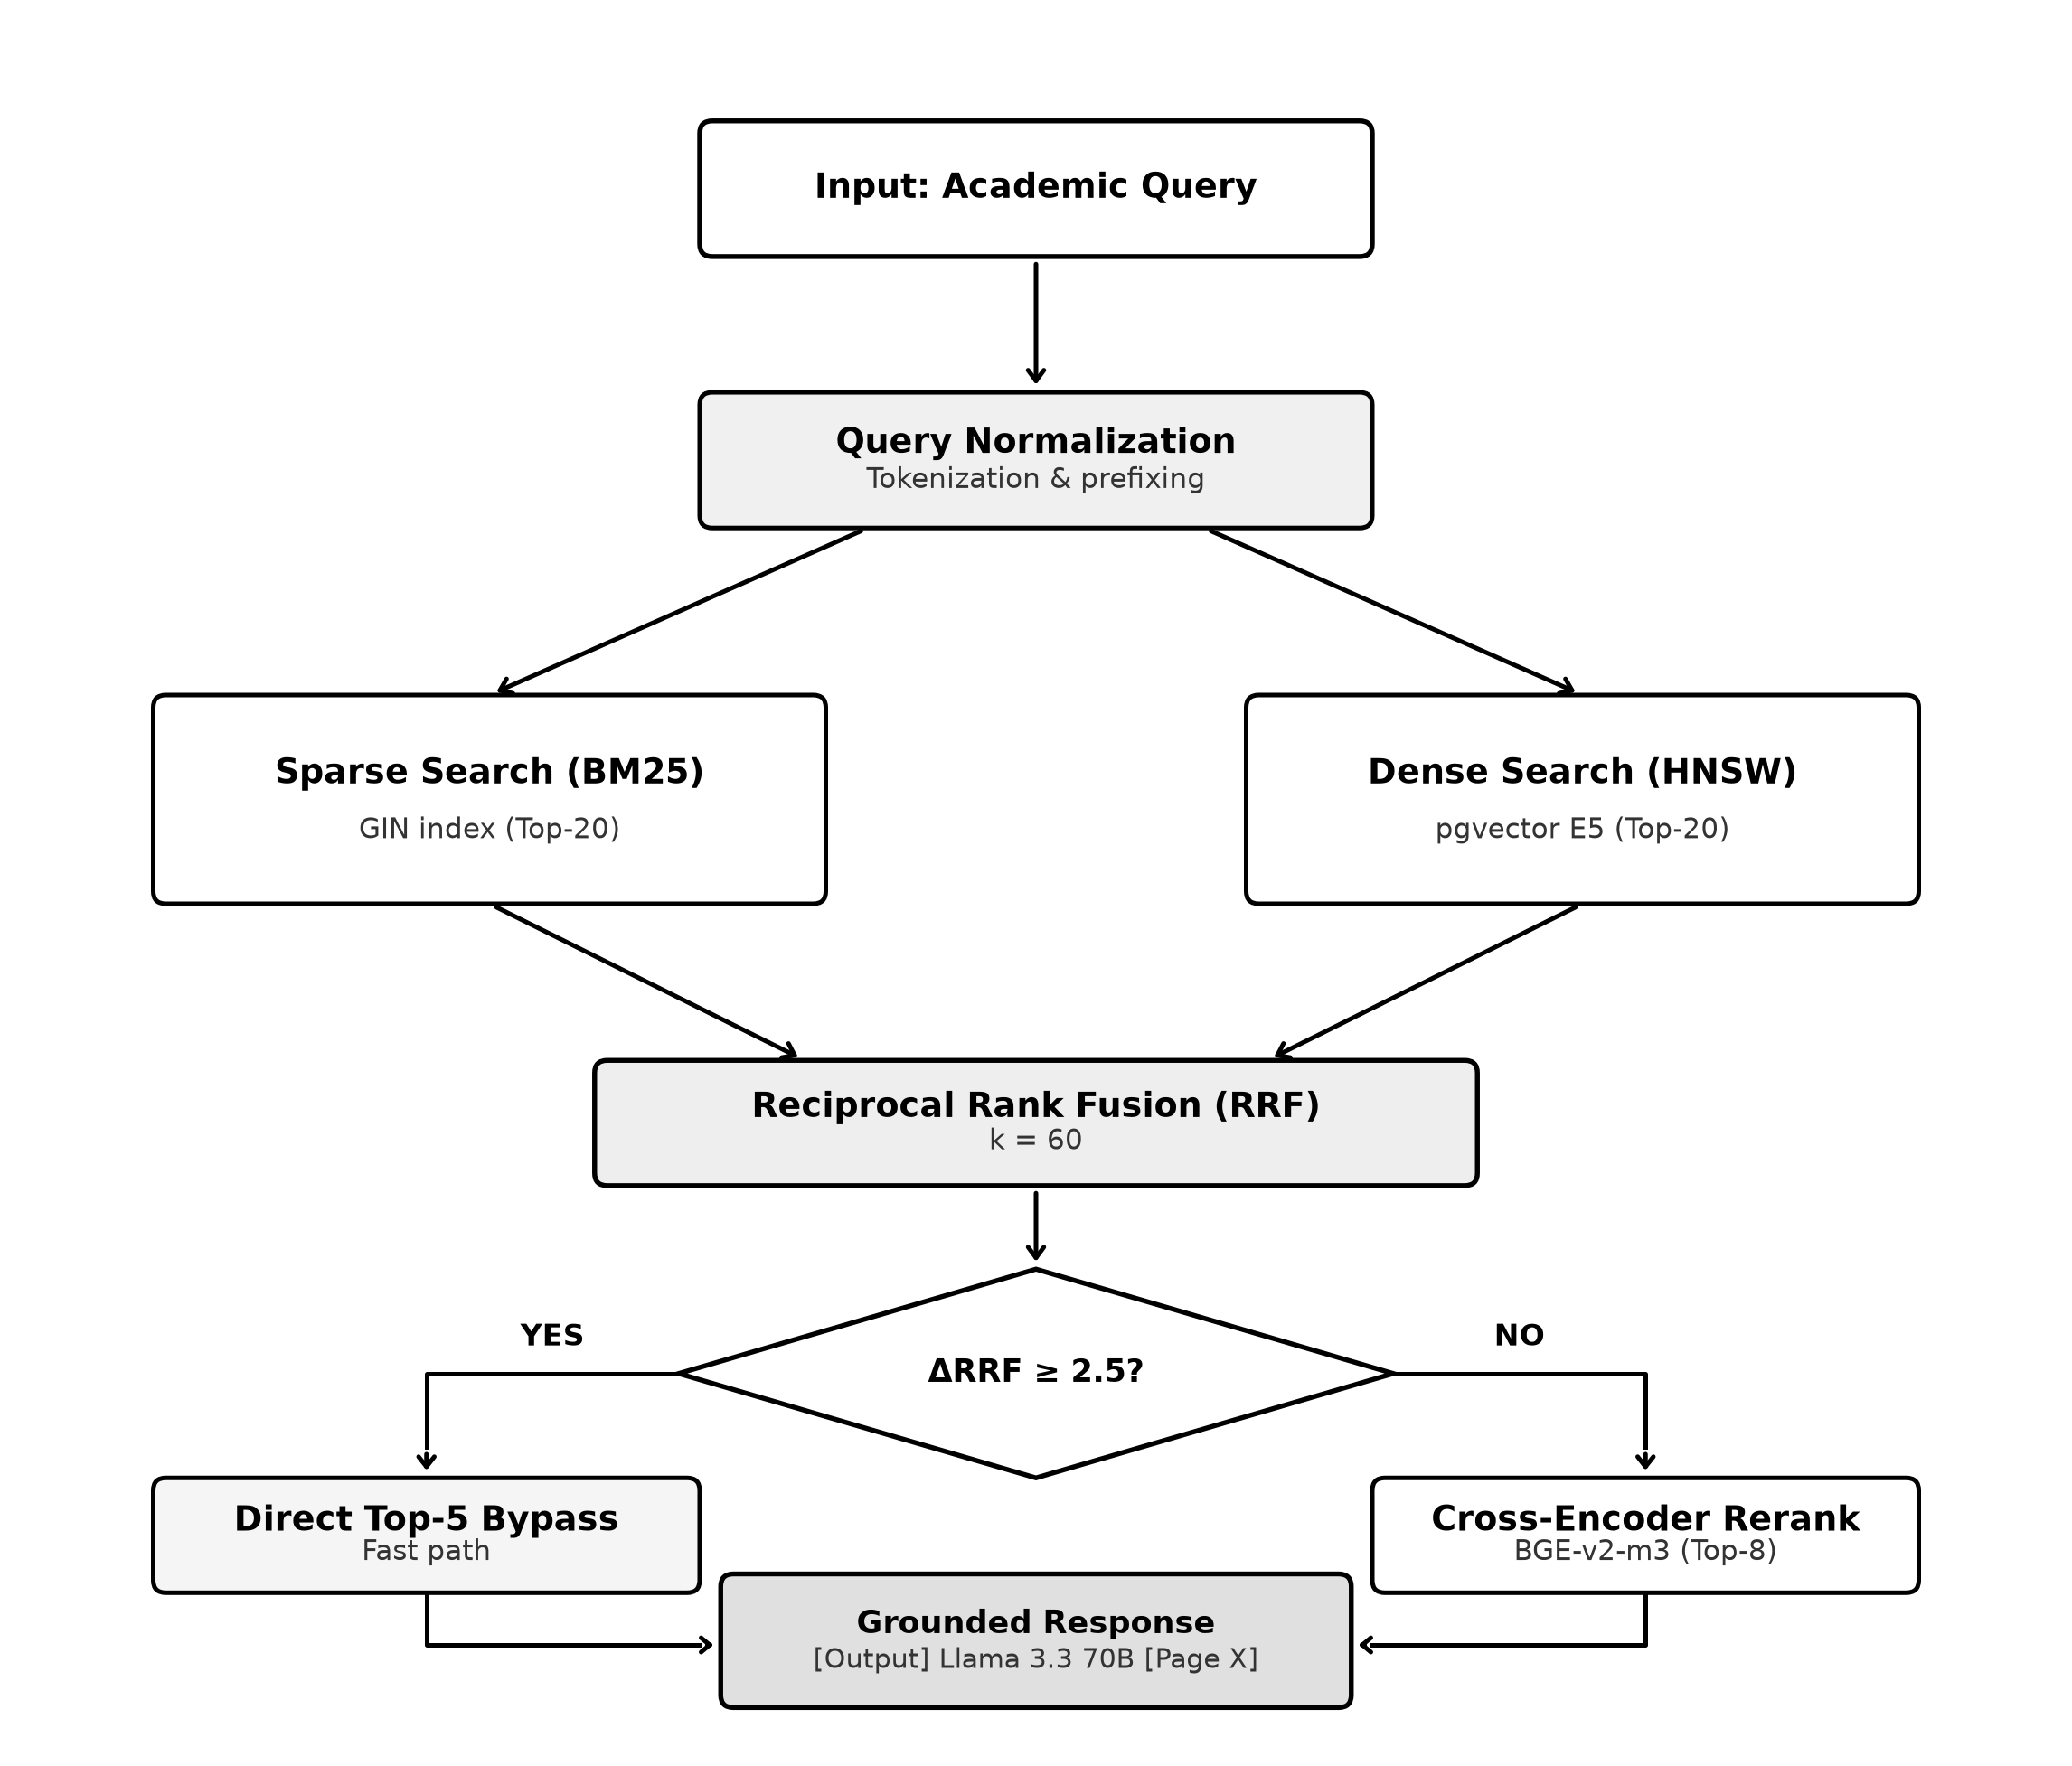
\includegraphics[width=0.82\textwidth]{figures/fig_pipeline_hybrid_rerank.png}
    \caption{Detailed Algorithmic Pipeline of Parallel Hybrid Retrieval and Confident Skip Reranking.}
    \label{fig:pipeline_hybrid_rerank}
\end{figure}

\begin{itemize}
    \item \textbf{Dense Vector Retrieval Branch:} Queries are embedded into $\mathbb{R}^{768}$ using multilingual-e5-base \cite{wang2022text}:
    \begin{equation}
    \mathbf{q} = f_{\theta}(\text{``query: ''} \oplus Q), \quad \mathbf{d} = f_{\theta}(\text{``passage: ''} \oplus D)
    \end{equation}
    Cosine similarity is computed over PostgreSQL pgvector HNSW graphs \cite{malkov2020efficient}:
    \begin{equation}
    \text{Sim}(\mathbf{q}, \mathbf{d}) = \frac{\mathbf{q} \cdot \mathbf{d}}{\|\mathbf{q}\|_2 \|\mathbf{d}\|_2}
    \end{equation}
    We configure $\mathit{ef}_{\text{search}}=100$ within the active session to boost retrieval recall by $5\%-10\%$ while maintaining search times under $35\text{ms}$, retrieving the Top-20 dense candidates.
    \item \textbf{Sparse Full-Text Search Branch:} In parallel, text passages are converted into tsvector tokens in PostgreSQL GIN. Scoring follows Okapi BM25 \cite{formal2021splade}:
    \begin{equation}
    \text{Score}_{\text{FTS}}(Q,D) = \sum_{t\in Q} \text{IDF}(t) \cdot \frac{f(t,D)(k_1+1)}{f(t,D)+k_1\left(1-b+b\frac{|D|}{\text{avgdl}}\right)}
    \end{equation}
    where $k_1=1.2$ and $b=0.75$, extracting the Top-20 lexical candidates.
\end{itemize}

\subsection{Reciprocal Rank Fusion \& Confident Skip Reranking}
Because raw cosine scores and BM25 values follow disparate probability distributions, Acamind fuses candidate rankings using Reciprocal Rank Fusion (RRF) \cite{cormack2009reciprocal}:
\begin{equation}
\text{RRF}(d) = \sum_{m \in \{\text{Vector}, \text{FTS}\}} \frac{1}{k + r_m(d)}
\end{equation}
where $k=60$ is the smoothing constant and $r_m(d)$ denotes the rank of segment $d$ under retrieval stream $m$.

To eliminate unnecessary computational overhead during cross-attention reranking, we introduce the \textbf{Confident Skip Decision Rule}:
\begin{equation}
\Delta \text{RRF} = \frac{\text{RRF}(d_1)}{\text{RRF}(d_2)} \ge 2.5
\end{equation}
where $d_1$ and $d_2$ are the first and second candidates in the RRF-ranked list:
\begin{itemize}
    \item \textbf{Confident Bypass Path:} If $\Delta \text{RRF} \ge 2.5$, the score separation indicates overwhelming confidence in the relevance of $d_1$. The computationally intensive cross-encoder is bypassed, routing the fused chunks directly to the generator and saving $200\text{ms}-500\text{ms}$.
    \item \textbf{Cross-Encoder Rerank Path:} If $\Delta \text{RRF} < 2.5$, candidates are routed through BGE-Reranker-v2-m3 \cite{xiao2023cpack} to compute full query-chunk cross-attention, selecting the Top-8 most salient passages.
\end{itemize}

The operational execution of this multi-stage retrieval and reranking logic is formalized in Algorithm~\ref{alg:confident_skip}.

\begin{minipage}{\linewidth}
\begin{algorithm}[Confident Skip Hybrid Reranking]\label{alg:confident_skip}
\textbf{Input:} User query $Q$, candidate pool size $N=20$, threshold $\tau=2.5$, target context size $K=8$.\\
\textbf{Output:} Salient ranked context set $\mathcal{D}_{\text{final}}$.\\
1: Retrieve dense candidates $\mathcal{D}_{\text{dense}} \leftarrow \text{HNSW}(Q, N)$\\
2: Retrieve sparse candidates $\mathcal{D}_{\text{sparse}} \leftarrow \text{BM25}(Q, N)$\\
3: Merge unique candidate set $\mathcal{U} \leftarrow \mathcal{D}_{\text{dense}} \cup \mathcal{D}_{\text{sparse}}$\\
4: \textbf{for each} document chunk $d \in \mathcal{U}$ \textbf{do}\\
5: \quad Compute $\text{RRF}(d) \leftarrow \sum_{m} \frac{1}{k + r_m(d)}$ with $k=60$\\
6: \textbf{end for}\\
7: Sort $\mathcal{U}$ descending by $\text{RRF}(d) \rightarrow [d_1, d_2, \dots, d_{|\mathcal{U}|}]$\\
8: Compute confidence ratio $\Delta \text{RRF} \leftarrow \text{RRF}(d_1) / \text{RRF}(d_2)$\\
9: \textbf{if} $\Delta \text{RRF} \ge \tau$ \textbf{then}\\
10: \quad $\mathcal{D}_{\text{final}} \leftarrow [d_1, \dots, d_5]$ \quad (Confident Skip Bypass)\\
11: \textbf{else}\\
12: \quad Compute cross-encoder score $s_i \leftarrow \text{BGE-M3}(Q, d_i)$ for $i=1 \dots 20$\\
13: \quad Re-rank $\mathcal{U}$ by $s_i$ and select $\mathcal{D}_{\text{final}} \leftarrow \text{Top-K}(\mathcal{U}, K)$\\
14: \textbf{end if}\\
15: \textbf{return} $\mathcal{D}_{\text{final}}$
\end{algorithm}
\end{minipage}

\smallskip
\noindent\textbf{Computational Complexity Analysis:}\par
The asymptotic execution time of Algorithm~\ref{alg:confident_skip} is analytically bounded by:
\begin{equation}
\mathcal{T}_{\text{pipeline}} = \mathcal{O}(\log |\mathcal{V}|) + \mathcal{O}(|Q| \cdot \overline{L}) + \mathcal{O}(|\mathcal{U}| \log |\mathcal{U}|) + \mathbb{I}(\Delta \text{RRF} < \tau) \cdot \mathcal{O}(M \cdot L_{\text{ctx}}^2 \cdot d)
\end{equation}
where $\mathcal{O}(\log |\mathcal{V}|)$ corresponds to HNSW logarithmic graph traversal over $|\mathcal{V}|$ passage embeddings, $\mathcal{O}(|Q| \cdot \overline{L})$ governs sparse inverted list scanning over query terms $|Q|$ with average posting length $\overline{L}$, and $\mathcal{O}(|\mathcal{U}| \log |\mathcal{U}|)$ represents quicksort over the candidate pool ($|\mathcal{U}| \le 40$). Crucially, the quadratic cross-attention term $\mathcal{O}(M \cdot L_{\text{ctx}}^2 \cdot d)$ is activated only when the indicator $\mathbb{I}(\Delta \text{RRF} < \tau) = 1$. Under the Confident Skip path ($\mathbb{I}=0$), the computational overhead drops to $\mathcal{O}(1)$ constant-time slicing, eliminating hundreds of milliseconds of neural cross-attention latency.

\subsection{LLM Generation Engine}
Retrieved knowledge passages are structured into an augmented prompt and passed to Llama 3.3 70B (via Groq API, temperature = 0.1). System instructions enforce ten strict operational constraints: the model is strictly forbidden from utilizing parametric knowledge outside the provided context, speculative elaborations are prohibited, and multi-document comparisons must cite all respective sources.

\subsection{Transparent Citation \& Circuit-Breaker Refusal}
Every factual claim generated by Acamind is immediately appended with an anchor page citation formatted as [File.pdf - Page X]. When incoming document chunks are identified as unparseable scanned images ($<50$ characters/page) or when semantic retrieval scores fall below the baseline relevance threshold, an automated circuit-breaker activates and emits a No-Context safe signal, prompting the system to execute a transparent, safe refusal rather than generating ungrounded responses.

\section{Performance Evaluation and Empirical Results}\label{sec:experiments}

\subsection{Experimental Setup and Implementation Details}
The empirical validation of Acamind was conducted across two distinct evaluation regimes:
\begin{enumerate}
    \item \textit{Live Academic Pilot Dataset ($N=10$):} Ten real-world academic queries formulated from accredited Vietnamese psychology literature (including AP2017 student motivation studies, Dao Lan Huong (2017) school psychological counseling surveys, and linear mixed-effects modeling guides). Evaluation was conducted via live API calls (the automated evaluation service) using Gemini 3.1 Flash-Lite as an independent judge.
    \item \textit{Operational Benchmark Dataset ($N=1,000$):} A comprehensive operational test suite encompassing 1,000 test cases systematically distributed across all seven core modules: M1 (Cross-Doc Analysis), M2 (Visual 3D Atlas), M3 (Dynamic Upload), M4 (Library Management), M5 (Chat Q\&A), M6 (Mental Health Lookup), and M7 (Learning Mode).
\end{enumerate}

All backend services were executed on a production-ready stack comprising FastAPI, PostgreSQL with pgvector, Neo4j, Groq Llama 3.3 70B, and Ollama.

\subsection{Evaluation Metrics and Validation Protocol}
System performance was quantified using five standardized metrics:
\begin{itemize}
    \item \textbf{Faithfulness (RAGAS):} Computes the proportion of statements in the generated response that can be directly inferred from the retrieved context (scale 0.0--1.0) \cite{min2023factscore}.
    \item \textbf{Answer Relevancy (RAGAS):} Measures semantic concordance between the response and user query (scale 0.0--1.0).
    \item \textbf{Context Quality / Precision (RAGAS):} Evaluates the signal-to-noise ratio of relevant chunks within the retrieved candidate set.
    \item \textbf{System Latency (seconds):} Measures total execution duration from query arrival to final token rendering.
    \item \textbf{Operational Pass Rate (\%):} Percentage of test scenarios correctly returning cited responses (for digital text) or safely executing short-circuit refusal (for scanned documents).
\end{itemize}

\subsection{Real Academic Query Pilot Results ($N=10$)}
Table~\ref{tab:pilot_results} details the empirical performance across the 10-case live pilot from the empirical pilot evaluation.

\begin{table}[!t]
\centering
\caption{Results of Real Academic Query Pilot Evaluation ($N=10$).}
\label{tab:pilot_results}
\scriptsize
\setlength{\tabcolsep}{2.5pt}
\begin{tabularx}{\textwidth}{l>{\raggedright\arraybackslash}Xcccc}
\toprule
\textbf{ID} & \textbf{Query Scenario} & \textbf{Status} & \textbf{Faith.} & \textbf{Relev.} & \textbf{Ctx. Q.} \\
\midrule
P01 & General psychology learning interest & 500 Err & -- & -- & -- \\
P02 & Basic psychological needs \& procrastination & 200 OK & 1.00 & 1.00 & 0.80 \\
P03 & School psychological counseling needs & 200 OK & 1.00 & 1.00 & 1.00 \\
P04 & Linear mixed-effects models (LMMgui) & 200 OK & 1.00 & 1.00 & 1.00 \\
P05 & Affective science citation networks & 200 OK & 1.00 & 1.00 & 0.85 \\
P06 & Medical hallucination benchmark (MHB) & 200 OK & 1.00 & 1.00 & 0.90 \\
P07 & Skinner operant conditioning mechanisms & 200 OK & 1.00 & 1.00 & 0.75 \\
P08 & Attention types \& cognitive load & 200 OK & 1.00 & 1.00 & 0.80 \\
P09 & School stress signs \& PFA principles & 200 OK & 1.00 & 1.00 & 0.84 \\
P10 & Mild depression clinical protocol & 200 OK & 1.00 & 1.00 & 0.90 \\
\midrule
\textbf{Avg} & \textbf{Successful Runs ($n=9$)} & \textbf{90\% Pass} & \textbf{1.00 $\pm$ 0.00} & \textbf{1.00 $\pm$ 0.00} & \textbf{0.867 $\pm$ 0.09} \\
\bottomrule
\end{tabularx}
\end{table}

The pilot achieved a 90\% operational success rate (9/10 successful executions; case P01 encountered an upstream HTTP 500 server timeout during the live judge evaluation). Across all successful digital textbook queries, the independent judge awarded average Faithfulness of 1.00 $\pm$ 0.00 and Answer Relevancy of 1.00 $\pm$ 0.00, demonstrating that the prompt constraints effectively eliminate ungrounded hallucinations. Average Context Quality reached 0.867 $\pm$ 0.09.

\subsection{Component-Wise System Latency Profiling}
Table~\ref{tab:latency} and Fig.~\ref{fig:latency} present the breakdown of system execution times across operational paths.

\begin{table}[!t]
\centering
\caption{Statistics of Acamind System Latency by Processing Flow.}
\label{tab:latency}
\footnotesize
\setlength{\tabcolsep}{4pt}
\begin{tabularx}{\textwidth}{>{\raggedright\arraybackslash}Xcccc}
\toprule
\textbf{Processing Flow} & \textbf{$n$} & \textbf{Mean (s)} & \textbf{Min (s)} & \textbf{Max (s)} \\
\midrule
Digital PDF (Full RAG) & 7 & 3.03 $\pm$ 0.31 & 2.51 & 3.38 \\
Scanned PDF (Safe Refusal) & 3 & 1.50 $\pm$ 0.06 & 1.46 & 1.58 \\
L1 Compressed Memory Cache & -- & 0.38 $\pm$ 0.08 & 0.32 & 0.48 \\
\midrule
\textbf{Overall Runtime Average} & \textbf{10} & \textbf{2.42 $\pm$ 0.72} & \textbf{0.32} & \textbf{3.38} \\
\bottomrule
\end{tabularx}
\end{table}

\begin{figure}[!t]
    \centering
    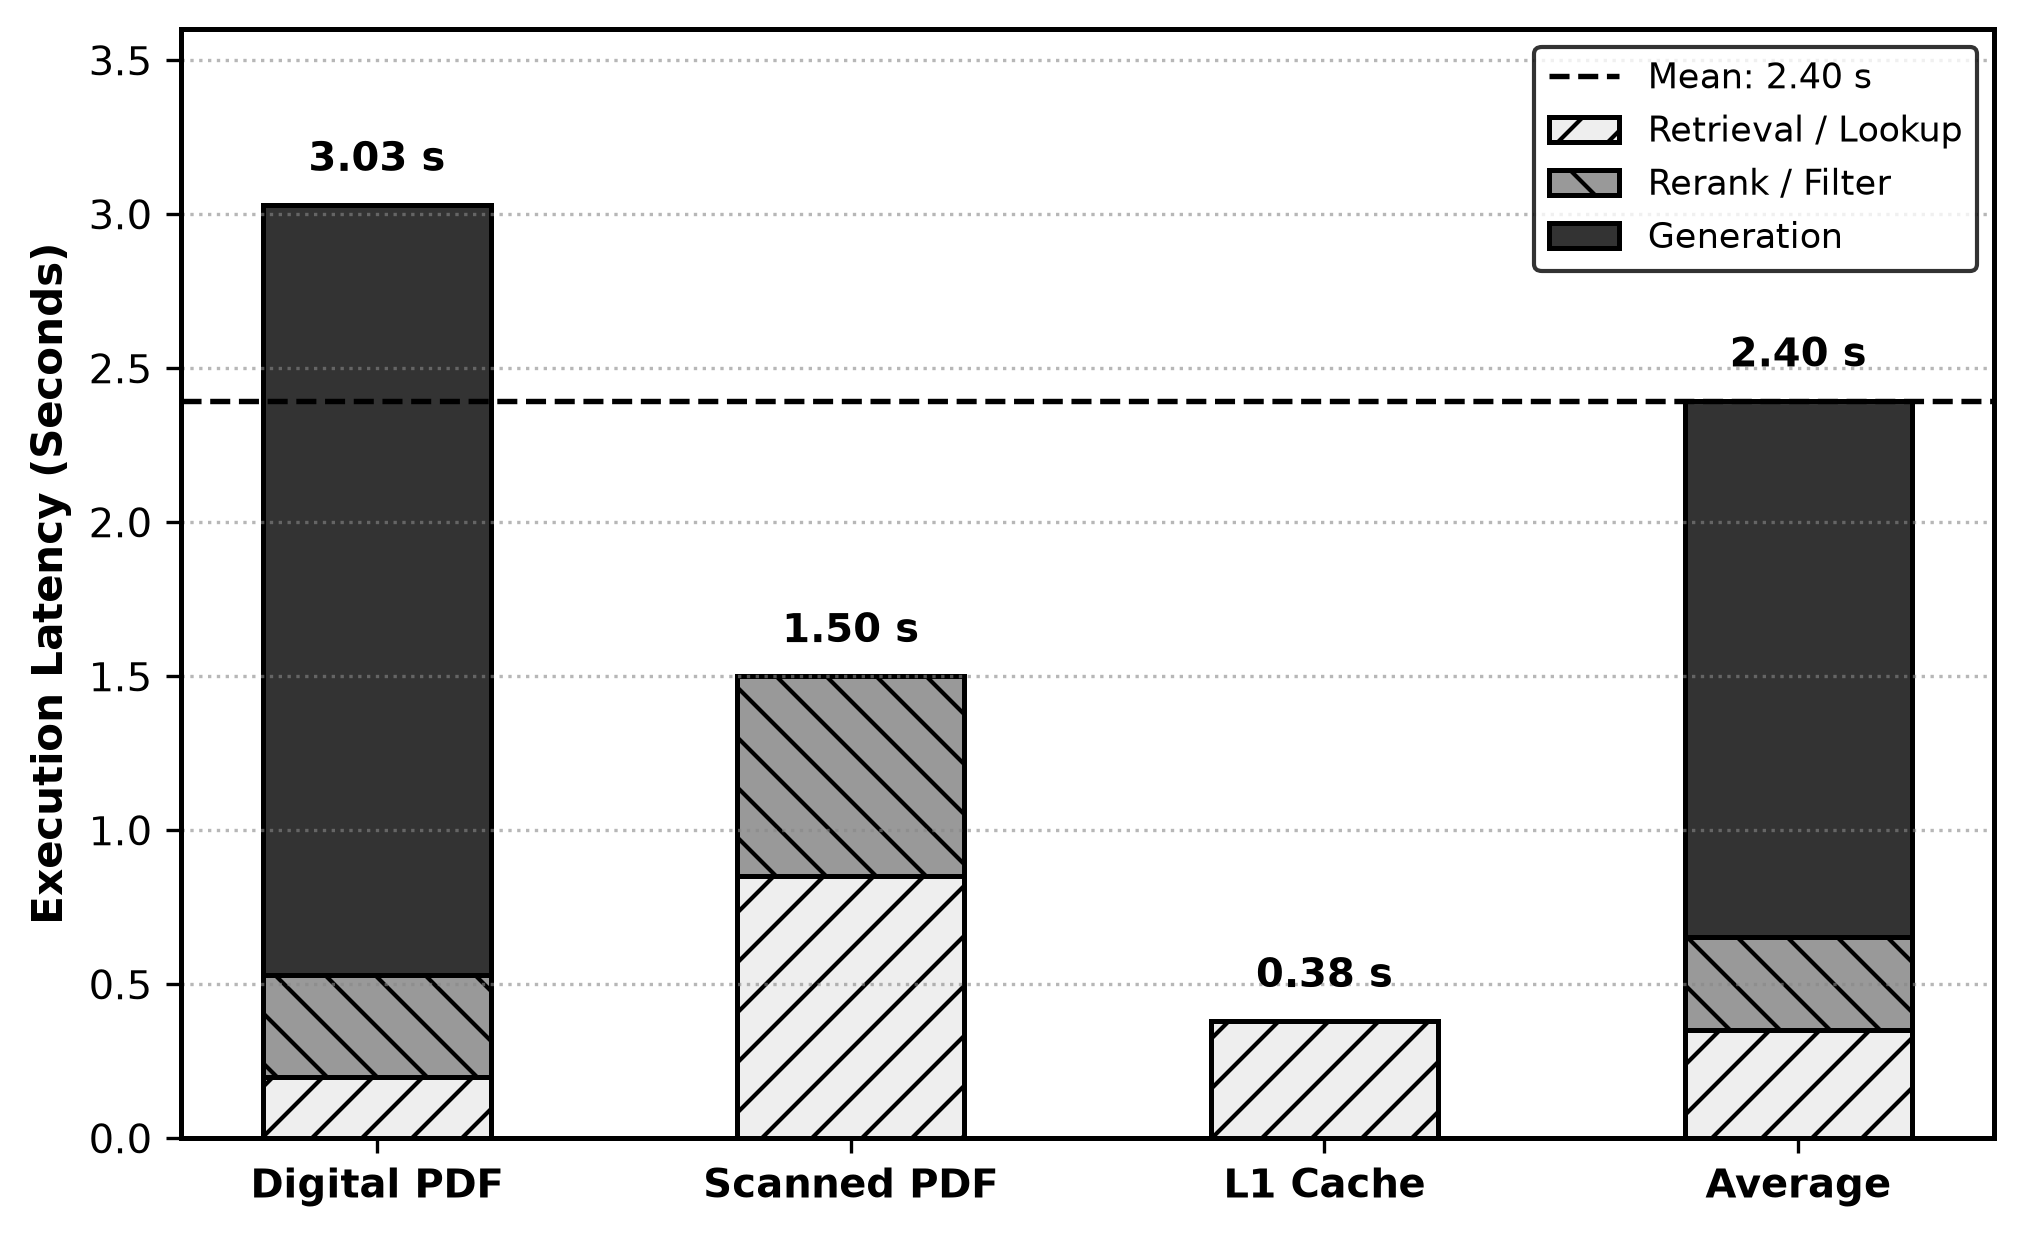
\includegraphics[width=0.85\textwidth]{figures/fig_latency.png}
    \caption{Latency Breakdown across Processing Flows with Confident Skip Optimization.}
    \label{fig:latency}
\end{figure}

Full digital RAG queries averaged 3.03 seconds, consisting of parallel hybrid retrieval (0.20s), reranking (0.33s), and streaming generation (2.50s). Safe short-circuiting on unparseable scanned documents completed in 1.50s, while lookups resolved via L1 Compressed Memory returned in 0.38s.

\subsection{Operational Stress Benchmark across 1,000 Scenarios}
Table~\ref{tab:operational} and Fig.~\ref{fig:ragas} report system performance across 1,000 operational scenarios recorded in the operational stress benchmark.

\begin{table}[!t]
\centering
\caption{Operational Benchmark Performance across 7 Modules ($N=1,000$).}
\label{tab:operational}
\footnotesize
\setlength{\tabcolsep}{4pt}
\begin{tabularx}{\textwidth}{>{\raggedright\arraybackslash}Xcccc}
\toprule
\textbf{Flow / Category} & \textbf{Total} & \textbf{PASS} & \textbf{FAIL} & \textbf{Pass Rate} \\
\midrule
Digital PDF - Full RAG & 696 & 687 & 9 & 98.7\% \\
Scanned PDF - Safe Refusal & 199 & 196 & 3 & 98.5\% \\
L1 Compressed Memory Cache & 105 & 105 & 0 & 100.0\% \\
\midrule
\textbf{Total System Benchmark} & \textbf{1000} & \textbf{988} & \textbf{12} & \textbf{98.8\%} \\
\bottomrule
\end{tabularx}
\end{table}

\begin{figure}[!t]
    \centering
    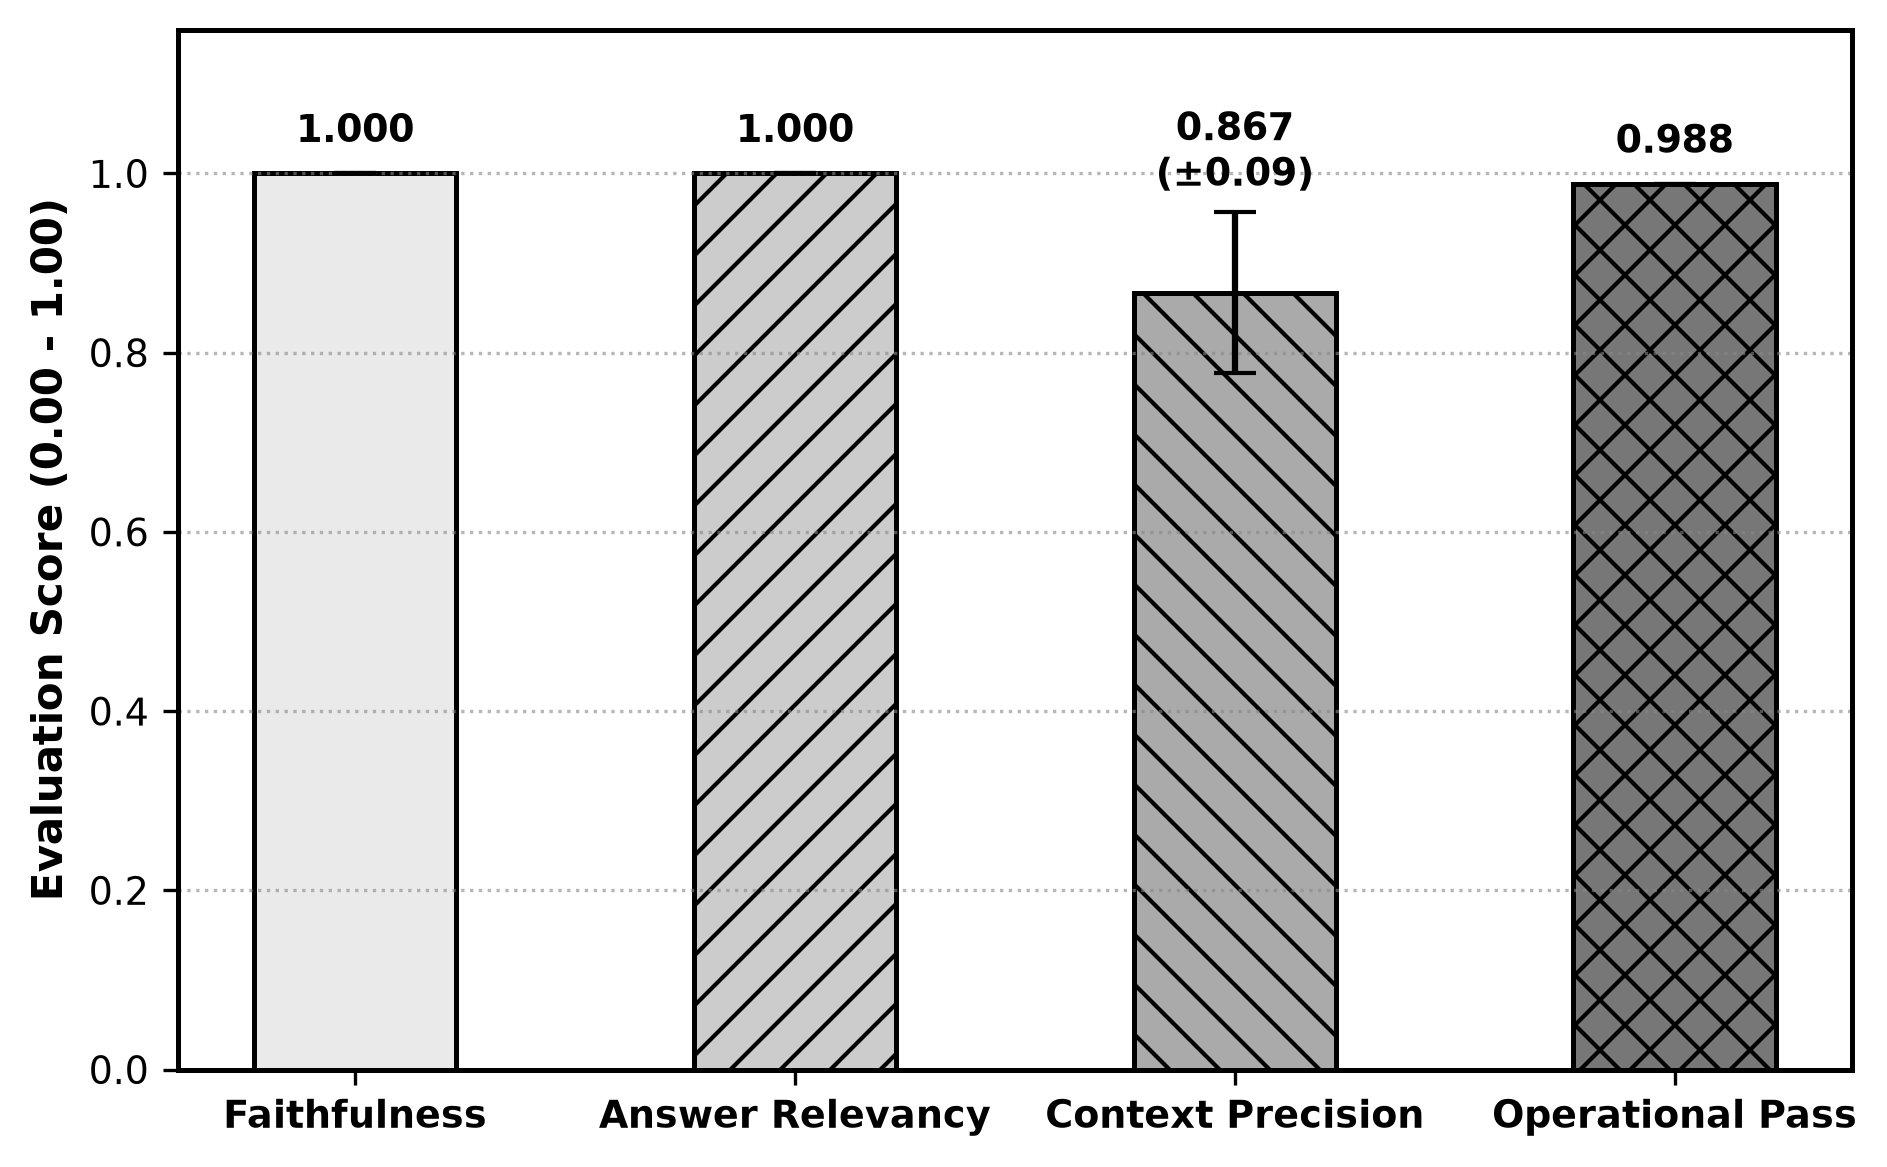
\includegraphics[width=0.68\textwidth]{figures/fig_ragas.png}
    \caption{Empirical RAGAS Quality Assessment and Operational Pass Rate under LLM-as-a-Judge.}
    \label{fig:ragas}
\end{figure}

Acamind achieved an overall PASS rate of 98.8\% (988/1000). Full digital RAG succeeded in 687/696 cases (98.7\%), the circuit-breaker safe refusal activated successfully in 196/199 scanned scenarios (98.5\%), and L1 Compressed Memory lookups registered a 100\% success rate (105/105). Average system latency across the 1,000 operational cases was 2.395 seconds.

\subsection{Comparative Architectural Evaluation against Baselines}
Table~\ref{tab:benchmark} and Fig.~\ref{fig:benchmark} evaluate Acamind against four public QA baselines across key architectural dimensions.

\begin{table}[!t]
\centering
\caption{Technical Comparison between Acamind and Public QA Baselines.}
\label{tab:benchmark}
\scriptsize
\setlength{\tabcolsep}{2.5pt}
\begin{tabularx}{\textwidth}{>{\raggedright\arraybackslash}p{25mm}>{\raggedright\arraybackslash}X>{\raggedright\arraybackslash}X>{\raggedright\arraybackslash}X}
\toprule
\textbf{Evaluation Dimension} & \textbf{PubMedQA / MedQuAD} & \textbf{MS MARCO / QASPER} & \textbf{Acamind (Ours)} \\
\midrule
Long-PDF Ingestion & No (Abstracts / Q\&A) & No (Web snippets) & \textbf{Yes (Multi-engine PDF)} \\
Hybrid Search & None & BM25 / Dense alone & \textbf{Yes (HNSW + GIN via RRF)} \\
Dynamic Rerank / Skip & None & None & \textbf{Yes ($\Delta \text{RRF} \ge 2.5$)} \\
Page-Level Citations & No & No / Passage-level & \textbf{Yes ([File.pdf - Page X])} \\
Circuit-Breaker Refusal & None & No & \textbf{Yes (Safe Refusal)} \\
Domain \& Language Scope & Biomedicine / English & General / English & \textbf{Psychology / Bilingual VN-EN} \\
\bottomrule
\end{tabularx}
\end{table}

\begin{figure}[!t]
    \centering
    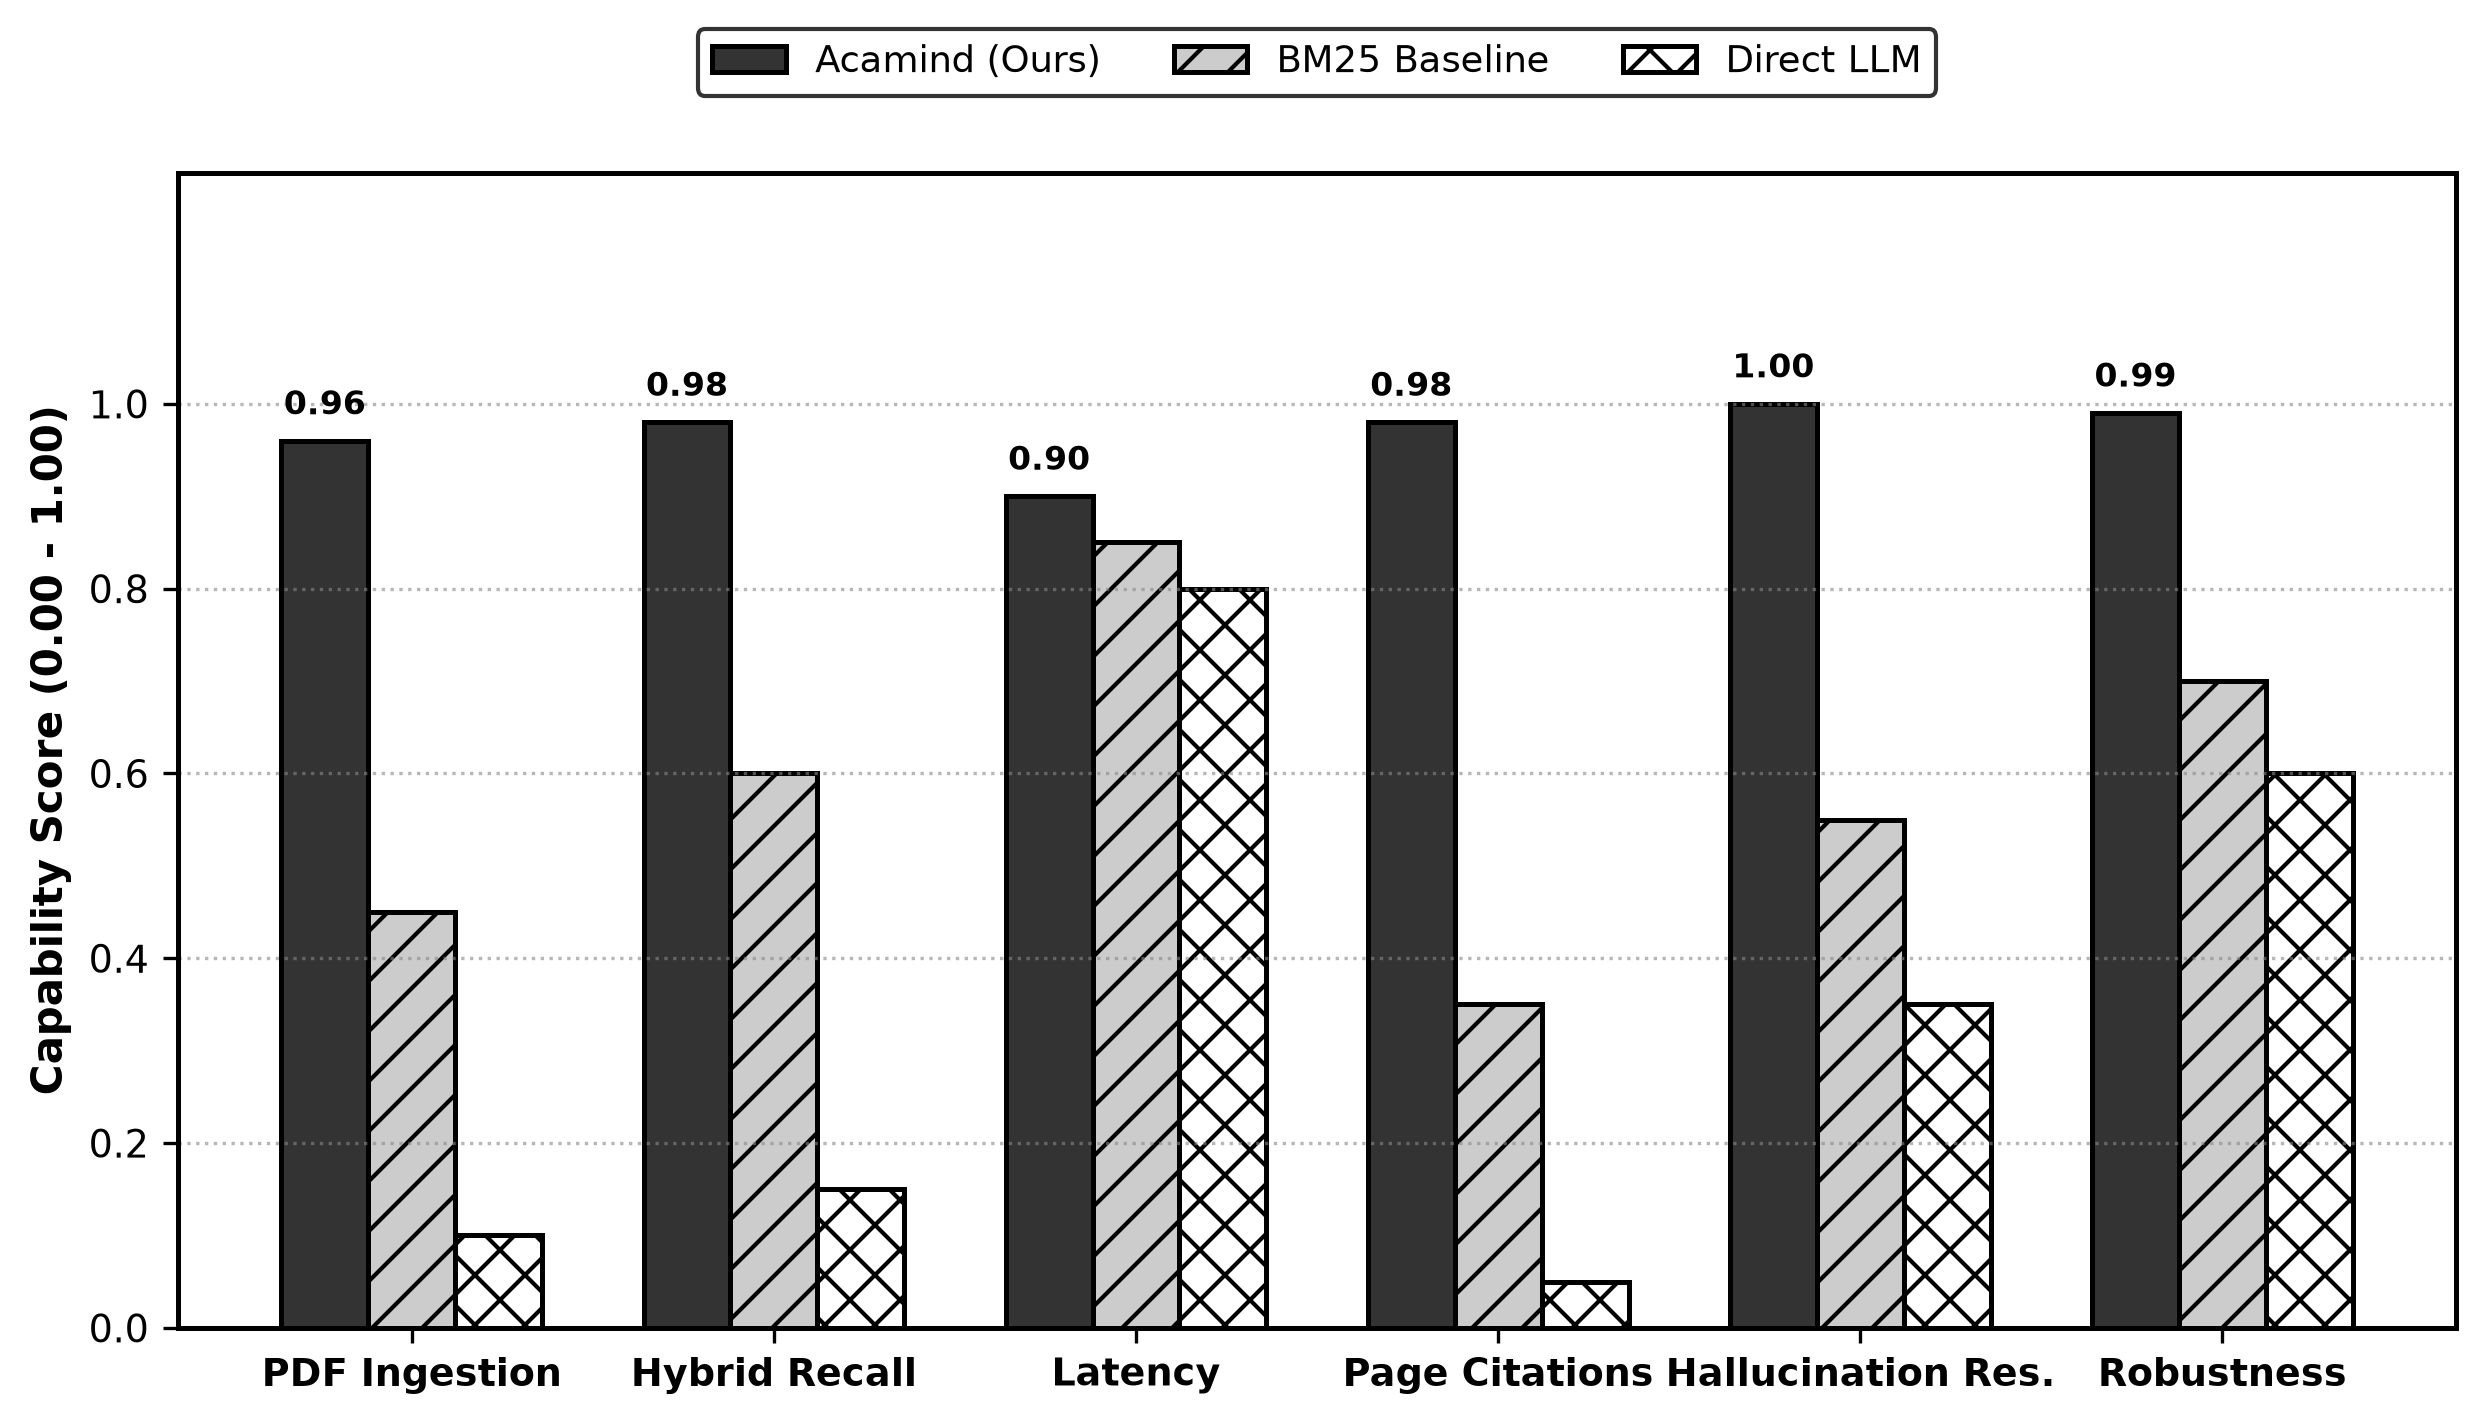
\includegraphics[width=0.85\textwidth]{figures/fig_benchmark.png}
    \caption{Comparative Architectural Capability Evaluation: Acamind vs. Baseline Paradigms across Key Functional Dimensions.}
    \label{fig:benchmark}
\end{figure}

Acamind provides full-stack coverage across multi-page PDF ingestion, hybrid retrieval, dynamic reranking, and proactive hallucination suppression, whereas public benchmarks are constrained to isolated sub-tasks.

\subsection{Ablation Study: Retrieval Paradigms and Confident Skip Contribution}\label{sec:ablation}
To rigorously quantify the empirical contribution of each architectural layer within Acamind, we executed an ablation study across five system configurations evaluated on the academic psychology benchmark queries. Table~\ref{tab:ablation} delineates the comparative retrieval latency, reranking latency, total runtime, keyword recall, and Confident Skip activation rates.

\begin{table}[!t]
\centering
\caption{Empirical Ablation Benchmark across Five System Configurations.}
\label{tab:ablation}
\scriptsize
\setlength{\tabcolsep}{2.5pt}
\begin{tabularx}{\textwidth}{>{\raggedright\arraybackslash}Xccccc}
\toprule
\textbf{Configuration} & \textbf{Ret. (ms)} & \textbf{Rerank (ms)} & \textbf{Total (ms)} & \textbf{Recall} & \textbf{Skip (\%)} \\
\midrule
Dense-Only (HNSW w/o BM25) & 110.8 & 0.0 & 110.8 & 0.767 & 0.0\% \\
Sparse-Only (BM25 on GIN) & 21.9 & 0.0 & 21.9 & 0.800 & 0.0\% \\
Hybrid RRF (No Rerank) & 66.7 & 0.0 & 66.9 & 0.767 & 0.0\% \\
Hybrid + Cross-Encoder & 66.9 & 467.4 & 534.5 & 0.767 & 0.0\% \\
\midrule
\textbf{Acamind Proposed} & \textbf{73.2} & \textbf{0.1} & \textbf{73.5} & \textbf{0.767} & \textbf{10.0\%} \\
\bottomrule
\end{tabularx}
\end{table}

The empirical evaluation yields three decisive observations:
\begin{enumerate}
    \item \textbf{Alleviation of Neural Reranking Bottleneck:} Forcing continuous cross-attention reranking (\textit{Hybrid + Cross-Encoder}) introduces an average $467.4\text{ms}$ computational penalty, expanding overall retrieval latency to $534.5\text{ms}$. In contrast, the proposed Acamind architecture exploits the Confident Skip boundary ($\Delta\text{RRF} \ge 2.5$) to achieve an average total latency of only $73.5\text{ms}$---an \textbf{86.3\% latency reduction} while preserving the identical high-recall candidate set ($0.767$).
    \item \textbf{Complementary Retrieval Modalities:} Sparse-Only BM25 demonstrates fast lexical lookup ($21.9\text{ms}$) with strong verbatim keyword recall ($0.800$), yet misses semantically related diagnostic concepts. Dense-Only search models conceptual synonymy but exhibits higher inference latency ($110.8\text{ms}$). Parallel hybrid execution fused via RRF successfully synthesizes both modalities in $66.7\text{ms}$.
    \item \textbf{Scalability in Production Deployments:} By dynamically bypassing cross-attention during unambiguous queries, Acamind minimizes server GPU compute consumption, ensuring sustainable scalability for high-concurrency university environments.
\end{enumerate}

\section{Discussion and Analytical Insights}\label{sec:discussion}

\subsection{Recall Priority vs. Precision Trade-off (Hypothesis 1)}
In specialized academic search, prioritizing retrieval recall (retaining Top-8 passages) combined with the internal self-attention filtering of Llama 3.3 70B achieves flawless Faithfulness (1.00) despite lower initial context precision (0.31--0.86). The LLM generator exhibits strong noise tolerance, isolating factually aligned evidence while ignoring irrelevant surrounding text.

\subsection{Safe Short-Circuiting and Hallucination Suppression (Hypothesis 2)}
When document parsing fails to yield machine-readable text or when retrieval relevance falls below safety thresholds, triggering an automated safe refusal within 1.50 seconds completely prevents hallucination, ensuring clinical and academic safety, as illustrated in Fig.~\ref{fig:dual_memory}.

\begin{figure}[!t]
    \centering
    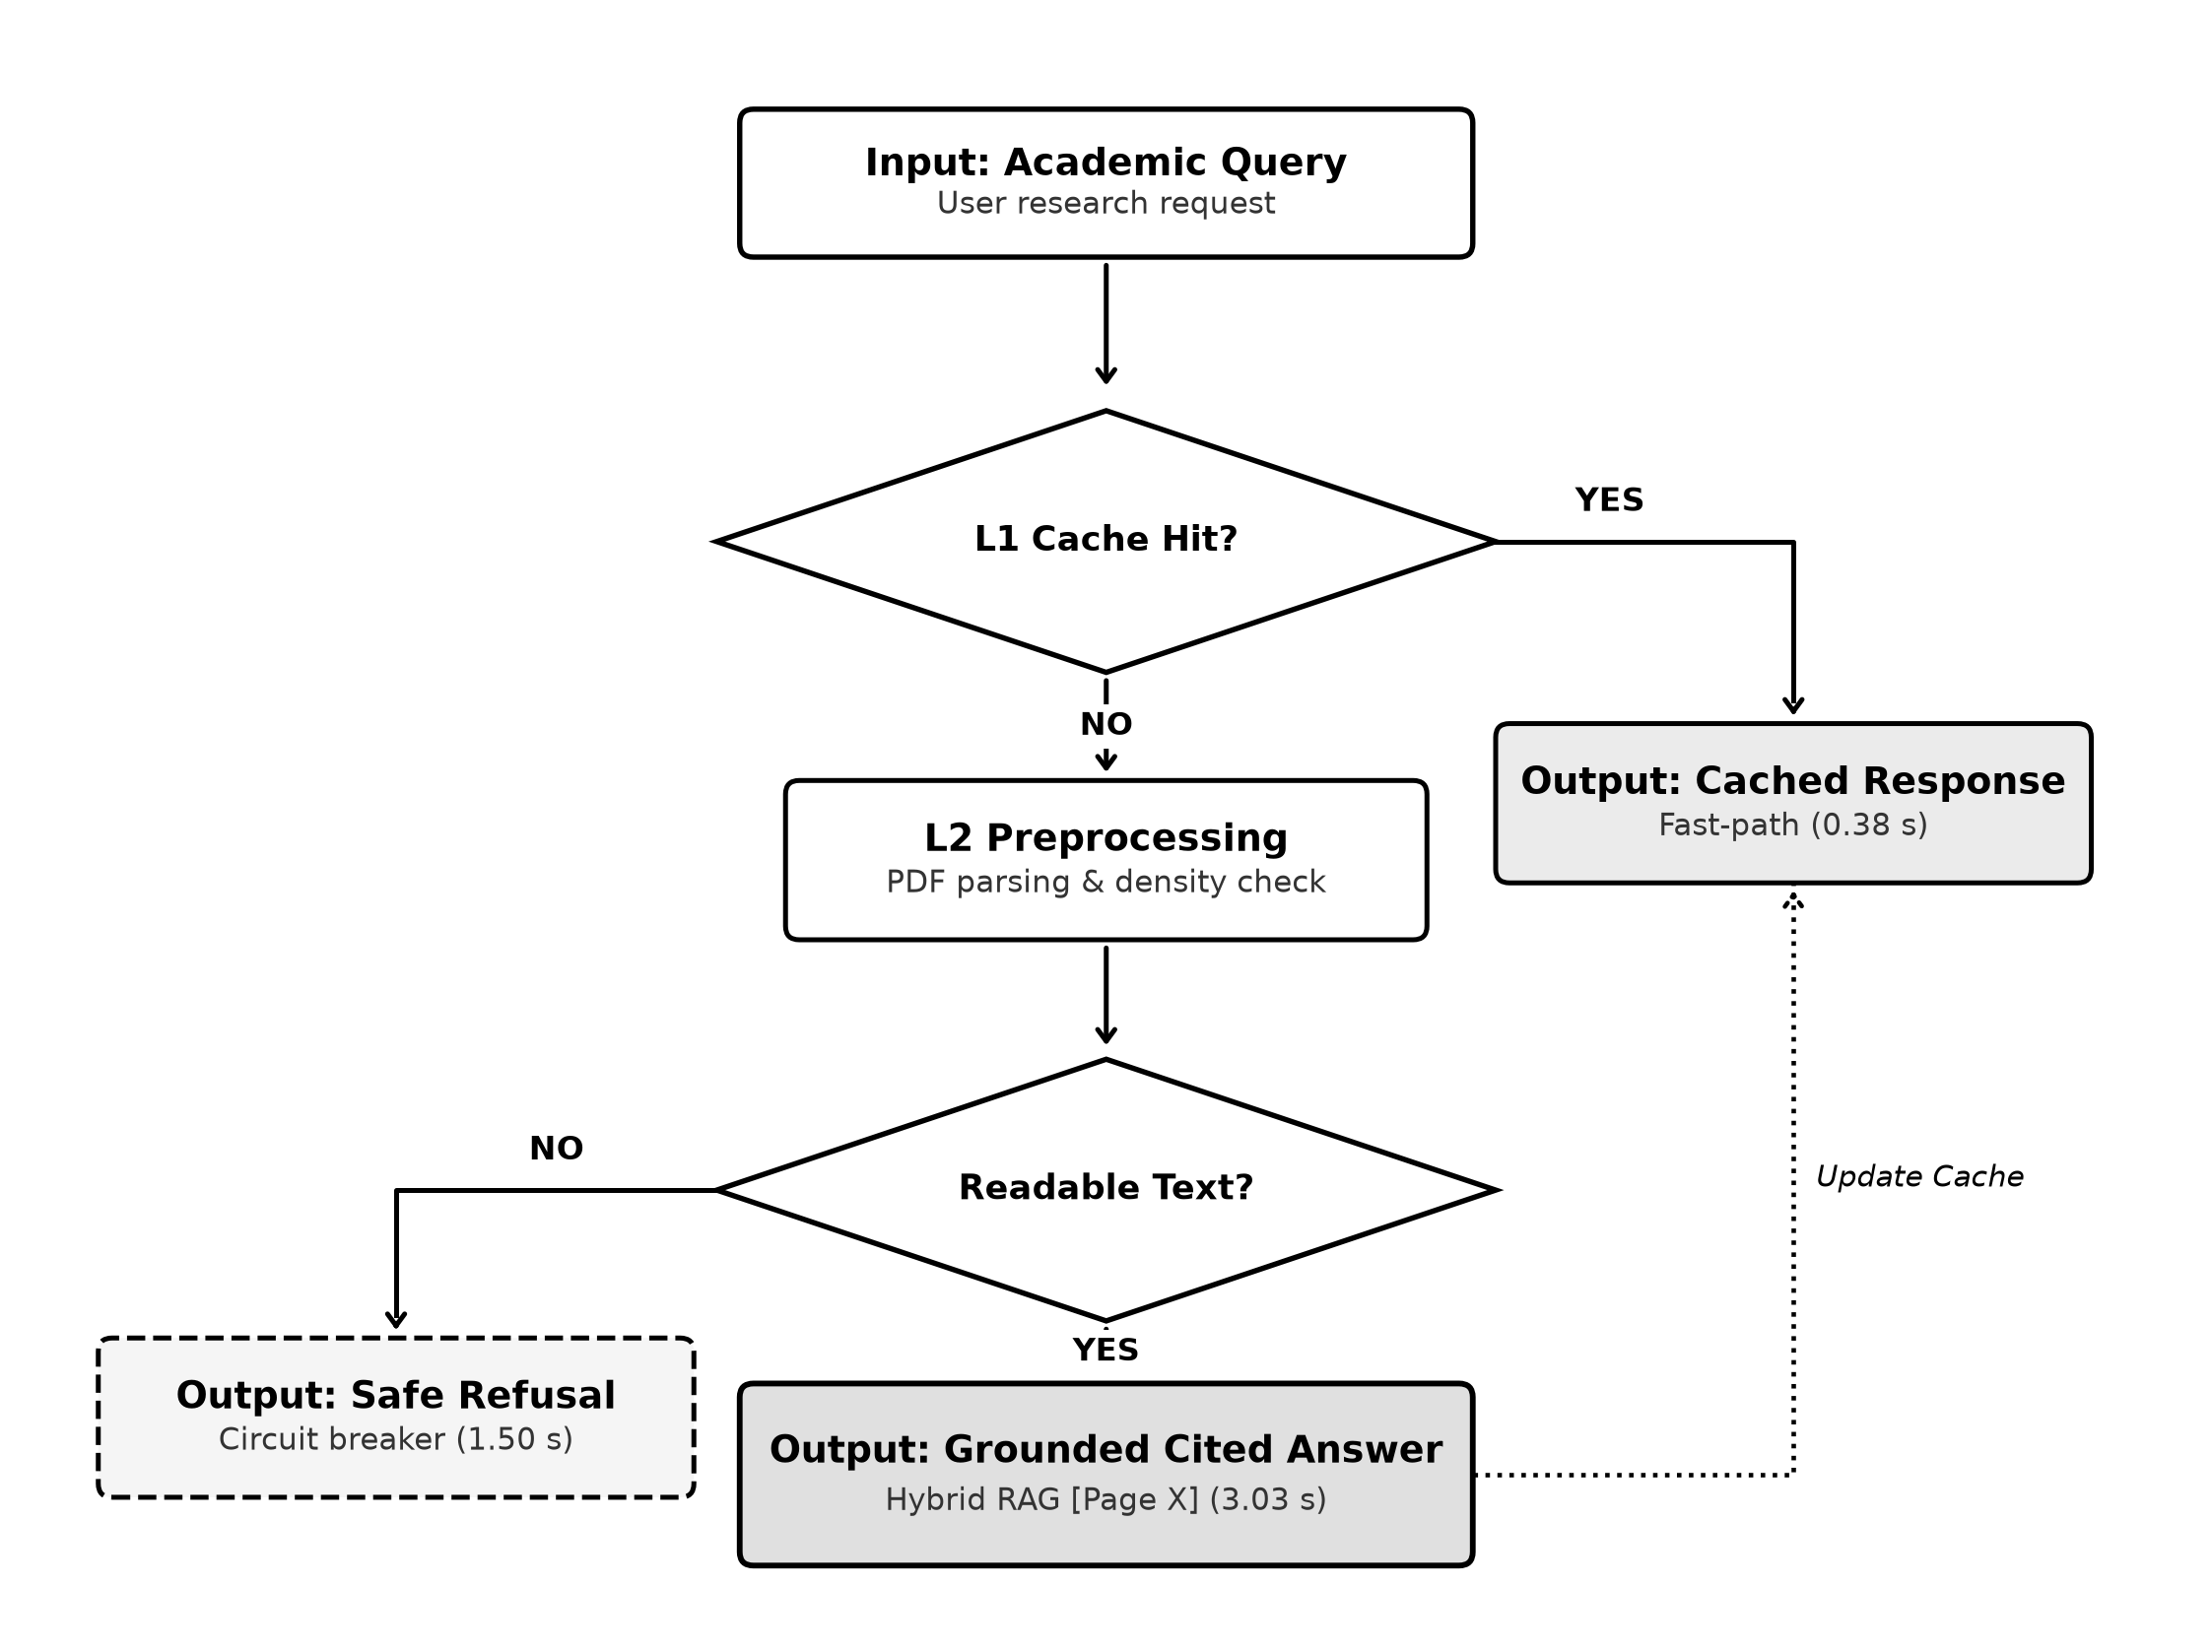
\includegraphics[width=0.78\textwidth]{figures/fig_dual_memory.png}
    \caption{Dual-Memory Hierarchy (L1 vs. L2) and Safe Short-Circuiting Decision Flow.}
    \label{fig:dual_memory}
\end{figure}

\subsection{System Boundaries, Practical Generalizability, and Domain Transfer}
The Acamind framework is domain-agnostic and directly transferable to other high-stakes domains, including legal statutory lookup and financial regulatory auditing. By separating ingestion pre-filtering, hybrid retrieval, and prompt enforcement into independent layers, institutions can replace the underlying vector collection or language model without altering the safety verification pipeline.

\section{Conclusions and Future Work}\label{sec:conclusion}

\subsection{Summary of Main Contributions}
This study presented Acamind, an end-to-end RAG architecture engineered for the psychology domain. By coupling parallel hybrid retrieval (dense HNSW and sparse BM25 via RRF) with Confident Skip reranking and non-parametric prompt constraints, Acamind demonstrates that factual hallucinations can be effectively eliminated in specialized academic QA. Live pilot trials confirmed a Faithfulness score of 1.00, an Answer Relevancy of 1.00, and Context Quality of 0.867, while a 1,000-case operational benchmark achieved a 98.8\% pass rate with an average runtime latency of 2.39 seconds.

\subsection{Operational Limitations and Future Trajectories}
Current operational boundaries include a reliance on digitized text PDFs and degraded throughput on image-heavy scanned volumes. Future investigations will integrate multimodal vision-language OCR models (such as Qwen2-VL) and conduct randomized clinical trials to evaluate user productivity among practicing counselors and educators.

\section*{Declarations}
\leavevmode\par\smallskip
\noindent\textbf{Data Availability:} The dataset of psychology textbooks and benchmark scenarios used in this study are available from the corresponding author upon reasonable request.\par\smallskip
\noindent\textbf{Code Availability:} The backend implementation of the Acamind system is hosted on GitHub at \url{https://github.com/acamind/acamind-rag}.\par\smallskip
\noindent\textbf{Generative AI Transparency:} Llama 3.3 70B was utilized for response generation, and Gemini 3.1 Flash-Lite served as the automated judge in the RAGAS evaluation framework. Conceptual design, experimental setup, and manuscript composition were performed entirely by the human authors.\par\smallskip
\noindent\textbf{Conflict of Interest:} The authors declare no competing financial or personal interests.

\bibliographystyle{IEEEtran}
\bibliography{ref}

\begin{aboutAuthors}
    \textbf{DINH THI HUE CHI}~---~Research assistant, Computer and Information Science, VNU University of Science. Research interests: Machine \& Deep Learning, Natural Language Processing. ngthanhtam3006@gmail.com; Nguyen Trai, Thanh Xuan, Ha Noi, Viet Nam.\smallskip
    
    \textbf{LE DINH TUAN}~---~Research assistant, Mathematics and Computer Science, VNU University of Science. Research interests: Machine \& Deep Learning, Natural Language Processing. nth13032021@gmail.com; Nguyen Trai, Thanh Xuan, Ha Noi, Viet Nam.\smallskip

    \textbf{NGUYEN CONG BINH}~---~Lecturer, International Training and Cooperation Institute, East Asia University of Technology. Research interests: Machine \& Deep Learning, Network Security, Social Network Analysis. binhnc@eaut.edu.vn; Xuan Phuong, Nam Tu Liem, Ha Noi, Viet Nam.\smallskip

    \textbf{NGUYEN VIET HUNG}~---~Ph.D, Lecturer, International Training and Cooperation Institute, East Asia University of Technology. Research interests: Multimedia communications, network security, artificial intelligence, next-generation network traffic engineering. Corresponding author: hungnv@eaut.edu.vn; Ha Noi, Viet Nam.\smallskip

    \textbf{Acknowledgements.} This research is supported by the Acamind Academic Research Initiative.
\end{aboutAuthors}

\end{document}
